\documentclass{article}
\usepackage{graphicx} 
\usepackage{float}
\usepackage{booktabs}
\usepackage{array}
\usepackage{arydshln}
\usepackage{siunitx}
\usepackage{hyperref}
\usepackage{cancel}
\usepackage{changepage}
\usepackage{placeins}
\usepackage{enumitem}
\usepackage{siunitx}
\usepackage{lipsum}
\usepackage[most]{tcolorbox}


%\usepackage{showframe}
\usepackage{times}

\DeclareSIUnit{\atm}{atm}

\usepackage{tabularx}
\usepackage{amsmath, amssymb, amscd, MnSymbol, mathrsfs}
\usepackage{cellspace}
\usepackage{tikz}
\usetikzlibrary{calc,3d, patterns, angles, quotes, decorations.markings, decorations.pathmorphing, hobby}
\usepackage{xfrac}

\usepackage{chemfig}
\usepackage{caption}
\usepackage{bm}
\usepackage{pdfpages}
\usepackage{empheq}
\usepackage{pgfplots}
\usepackage{pgfplotstable}
\usepackage{xstring}

\pgfplotsset{compat=1.18}
\usepackage[oldvoltagedirection]{circuitikz}
\usepackage{microtype}
\usepackage{tikz-3dplot}
\usepackage{textcomp}
% Custom commands
\newcommand{\vect}[1]{\boldsymbol{\mathbf{#1}}}
\newcolumntype{C}{>{\centering\arraybackslash}X}
\newcolumntype{M}[1]{>{\centering\arraybackslash}m{#1}}

\usetikzlibrary{external}
\tikzexternalize[prefix=figures/]

\newcommand\myfrac[2]{\sfrac{#1\mkern-1.2mu}{#2}}
\usepackage{xcolor}

% Define custom colors
\definecolor{darkblue}{rgb}{0.1,0.1,0.5} % A dark blue shade
\definecolor{formalshade}{rgb}{0.95,0.95,1} % A light blue shade for the background

% For the adjustwidth environment
\PassOptionsToPackage{strict}{changepage}
\usepackage{changepage}

% For formal definitions
\usepackage{framed}

\newcommand{\formalsource}{} % Initialize an empty macro to store the source text

\newenvironment{formal}[3][]{% Start of the environment
	\renewcommand{\formalsource}{#1}% Store the optional argument
	\def\FrameCommand{%
		\hspace{1pt}%
		{\color{#2}\vrule width 2pt}%
		{\color{#3}\vrule width 4pt}%
		\colorbox{#3}%
	}%
	\MakeFramed{\advance\hsize-\width\FrameRestore}%
	\noindent\hspace{-4.55pt}% Disable indenting the first paragraph
	\begin{adjustwidth}{}{7pt}%
		\vspace{2pt}%
	}%
	{%
		\vspace{4pt}%
		\ifx\formalsource\empty % Check if the source is empty
		\else
		\hfill{\footnotesize{\formalsource}}% Align source to the bottom-right
		\fi
	\end{adjustwidth}\endMakeFramed%
}


% Custom itemize list with images for positive and negative items
\newlist{gitemize}{itemize}{1} % Just one level for the list
\setlist[gitemize,1]{
	leftmargin=2.8em, % Adjust the margin for the list
	labelsep=1em % Control the space between the label and the list item
}

% Define checkmark and cross symbols for positive and negative items
\newcommand{\checkitem}{\raisebox{-0.25\height}{\includegraphics[width=0.4cm]{checkmark.png}}}
\newcommand{\crossitem}{\raisebox{-0.25\height}{\includegraphics[width=0.4cm]{cross.png}}}


\usepackage[left=0.8in,right=0.8in,top=0.5in,bottom=0.69in,includeheadfoot,letterpaper]{geometry}
\usepackage{fancyhdr}
\usepackage{graphicx}
\usepackage{tabularray}
\usepackage{varwidth} 


\newcommand{\wm}[2]{%
	\begin{minipage}{#1\textwidth}
		\centering
		#2
	\end{minipage}%
}

\pagestyle{fancy}
\fancyhf{}


\renewcommand{\headrulewidth}{0.4pt}
\renewcommand{\footrulewidth}{0.4pt}

\fancyhead[L]{\includegraphics[height=1.2cm]{images/Kingston_University_London_logo_200-tablet.png}}
\fancyhead[R]{EG4024 – ME – Fluid Mechanics and Thermodynamics}
\fancyfoot[C]{Department of Mechanical Engineering}
\fancyfoot[R]{\thepage}

\usepackage{scalerel}
\usepackage{pythonhighlight}
\setlength{\headheight}{30pt}
\setlength{\footskip}{20pt}



\usepackage[export]{adjustbox}
\usepackage{tocloft}
\renewcommand{\cfttoctitlefont}{}
\renewcommand{\contentsname}{}
\renewcommand{\cftsecleader}{\cftdotfill{\cftdotsep}}

\setlength{\cftbeforesecskip}{0.5em}



\usepackage{hyperref}    % For hyperlinks
\usepackage{xurl}        % For better URL handling
\hypersetup{
	colorlinks=true,
	linkcolor=blue!50!black,
	urlcolor=blue,       % Color for URLs
}


\definecolor{ChineseGold}{HTML}{C59401}
\definecolor{AmericanGold}{HTML}{D3AF37}
\definecolor{MetallicSunburst}{HTML}{A77C37}
\definecolor{GoldenBrown}{HTML}{996515}
\definecolor{DarkBrown}{HTML}{674222}
\definecolor{SkyBlue}{HTML}{87CEEB}      % Soft and bright
\definecolor{BabyBlue}{HTML}{89CFF0}     % Gentle, pastel-like
\definecolor{SteelBlue}{HTML}{4682B4}    % Rich but not overpowering
\definecolor{RoyalBlue}{HTML}{4169E1}    % Strong, slightly purplish
\definecolor{MidnightBlue}{HTML}{191970} % Almost black, deep navy
\definecolor{PrussianBlue}{HTML}{003153} % Very deep blue with a classic look


\usepackage{listings}

\definecolor{codegreen}{rgb}{0,0.6,0}
\definecolor{codegray}{rgb}{0.5,0.5,0.5}
\definecolor{codepurple}{rgb}{0.58,0,0.82}
\definecolor{backcolour}{rgb}{0.95,0.95,0.92}

\lstdefinestyle{mystyle}{
	backgroundcolor=\color{white!97!gray},   
	commentstyle=\color{codegreen},
	keywordstyle=\color{purple},
	numberstyle=\tiny\color{codegray},
	stringstyle=\color{orange},
	basicstyle=\ttfamily\scriptsize,
	breakatwhitespace=false,         
	breaklines=true,                 
	captionpos=b,                    
	keepspaces=true,                 
	numbers=left,                    
	numbersep=5pt,                  
	showspaces=false,                
	showstringspaces=false,
	showtabs=false,                  
	tabsize=2
}

\lstset{style=mystyle}

%Refer to the equation as \eqref{equation}.
\usepackage{caption}  % This package allows captioning outside of a float
\usepackage[export]{adjustbox}


\usetikzlibrary{patterns}

\usetikzlibrary{patterns.meta}
\usepackage[para]{footmisc} % Example of making footnotes run together in a paragraph

\definecolor{darkgreen}{rgb}{0.0, 0.5, 0.0}

\usepackage{datetime}

\usepackage{etoolbox}

\makeatletter
\def\tagform@#1{\maketag@@@{{Eq.~#1}}} 
\makeatother

\usepackage{ifthen}
\usepackage{calc}
\usepackage{datenumber}

\usepackage{physics}
\usepackage[outline]{contour}
\usetikzlibrary{patterns,decorations.pathmorphing}
\usetikzlibrary{arrows.meta}
\tikzset{>=latex}
\contourlength{1.1pt}

\colorlet{mydarkblue}{blue!50!black}
\colorlet{myred}{red!65!black}
\colorlet{watercol}{blue!80!cyan!10!white}
\colorlet{darkwatercol}{blue!80!cyan!20!white}
\tikzstyle{piston}=[blue!50!black,top color=blue!30,bottom color=blue!50,middle color=blue!20,shading angle=0]
\tikzstyle{water}=[draw=mydarkblue,top color=watercol!90,bottom color=watercol!90!black,shading angle=5]
\tikzstyle{vertical water}=[water,
top color=watercol!90!black!90,bottom color=watercol!90!black!90,middle color=watercol!80,shading angle=90]
\def\tick#1#2{\draw[thick] (#1)++(#2:0.1) --++ (#2-180:0.2)}


% Initialize counters
\newcounter{deadlineyear}\setcounter{deadlineyear}{2025}
\newcounter{deadlinemonth}\setcounter{deadlinemonth}{4}
\newcounter{deadlineday}\setcounter{deadlineday}{3}
\newcounter{mydatenumber}
\newcounter{currentdate}
\newcounter{daysdiff}
\newcounter{currenttime}
\newcounter{totalminutes}
\newcounter{displaydays}
\newcounter{remainingmins}
\newcounter{displayhours}
\newcounter{displaymins}

% Main calculation command
\newcommand{\timeUntilDeadline}{%
	% Calculate days between dates
	\setmydatenumber{mydatenumber}{\thedeadlineyear}{\thedeadlinemonth}{\thedeadlineday}%
	\setmydatenumber{currentdate}{\the\year}{\the\month}{\the\day}%
	\setcounter{daysdiff}{\themydatenumber - \thecurrentdate}%
	
	% Get current time in minutes since midnight
	\setcounter{currenttime}{\time}%
	
	% Calculate total remaining minutes
	\setcounter{totalminutes}{\numexpr\thedaysdiff * 1440 - \thecurrenttime}%
	
	% Check deadline status
	\ifnum\thetotalminutes < 0
	\textbf{\color{red}Deadline passed!}%
	\else
	% Calculate time components
	\setcounter{displaydays}{\thetotalminutes / 1440}%
	\setcounter{remainingmins}{\numexpr\thetotalminutes - \thedisplaydays * 1440}%
	\setcounter{displayhours}{\theremainingmins / 60}%
	\setcounter{displaymins}{\numexpr\theremainingmins - \thedisplayhours * 60}%
	
	% Format output
	\textbf{%
		\ifnum\thedisplaydays > 0
		\thedisplaydays\ day\ifnum\thedisplaydays > 1 s\fi%
		\ifnum\thedisplayhours > 0
		\ifnum\thedisplaymins > 0, \else\ and \fi%
		\else
		\ifnum\thedisplaymins > 0\ and \fi%
		\fi%
		\fi%
		\ifnum\thedisplayhours > 0
		\thedisplayhours\ hour\ifnum\thedisplayhours > 1 s\fi%
		\ifnum\thedisplaymins > 0\ and \fi%
		\fi%
		\ifnum\thedisplaymins > 0
		\thedisplaymins\ minute\ifnum\thedisplaymins > 1 s\fi%
		\fi%
		\ left}%
	\fi
}

\definecolor{mygreen}{HTML}{07a56d}

\newtcbtheorem{briefillus}{Definiton}{
	enhanced,
	sharp corners,
	attach boxed title to top left={
		xshift=0pt, 
		yshift=-\tcboxedtitleheight, 
		yshifttext=-\tcboxedtitleheight/2-0.5em
	},
	colback=white,
	colframe=black,
	fonttitle=\bfseries,
	coltitle=white,
	boxed title style={
		rounded corners,
		arc=2pt,
		size=small,
		colback=black,
		colframe=black,
	},
	leftrule=0pt, 
	rightrule=0pt, 
}{thm}



\newcounter{dataset}

% 2. Create a custom environment
\newenvironment{datasetbox}[2]{
	\refstepcounter{dataset}
	\begin{tcolorbox}[
		title={\color{black}\textbf{Dataset \thedataset: #1}},
		colback=black!4!white,
		colframe=black!10!white,
		boxrule=0.5mm,
		width=\textwidth,
		label={#2}]
	}{\end{tcolorbox}}


\usepackage{multirow}

\begin{document}
	
	\vspace*{\fill}
	\begin{center}
		\textbf{\Huge Laboratory Report}\\[10pt]
		\LARGE \textbf{Pressure}
	\end{center}
	\vspace*{\fill}
	
	\Large    
	\begin{tabular}{@{}l l l@{}}
		\textbf{Submitted by:} & Sakariye Abiikar (Group Leader) & K2371673 \\
		& Alireza Alishahi & K2333243 \\
		& Naim Alrifai & K2459662 \\
		& Munachi J Atuegbu & K2463699 \\
		& Ehsan Haque & K2453799 \\
		& Abdul Mueed & K2454880 \\   
		& Abdelrahman Shehata & K2426523 \\   
		& Varley, Freddie & K2311322
	\end{tabular}
	
	\vspace*{\fill}
	
	\begin{tabular}{@{}l l@{}}
		\textbf{Key Dates:} & Date of practical: Wednesday 19$^{\text{th}}$ March, 2025 \\
		& Deadline: Thursday 3$^{\text{rd}}$ April, 2025 \\
		& Last Updated: \today\, \currenttime
		%Days left until deadline: \timeUntilDeadline \\
	\end{tabular}
	\vspace*{\fill}
	
	\large
	\newpage\noindent	\vspace*{-1em}
	
	\begin{center}
		\LARGE \textbf{Contribution Table}\\[1.2em]
	\end{center}	
	
	
	\begin{tblr}{
			colspec={Q[4cm]Q[4cm]Q[4cm]Q[3cm]},
			hlines,vlines,
			cells={valign=m,halign=c},
			rows={ht=4\baselineskip},
			row{1}={ht=1.5\baselineskip,font=\bfseries},
			row{Z}={bg=black!5!white},
			row{8}={bg=red!5!white}
		}
		Student & Course & Contribution & Picture \\ 
		Sakariye Abiikar & Mechanical Engineering & Formatter, Data Calculation and Results, Introduction, & \includegraphics[width=2cm,valign=c]{images/image(7).jpg} \\ 
		Alireza Alishahi & Mechanical Engineering  & Abstract, Method \& Experimental Procedures & 
\includegraphics[width=2cm,valign=c]{images/8_orgid_297f9608-cce6-40e3-adc2-86e161e7141f.jpg} \\ 
		Varley, Freddie & Mechanical Engineering & Theory, Recommendations &  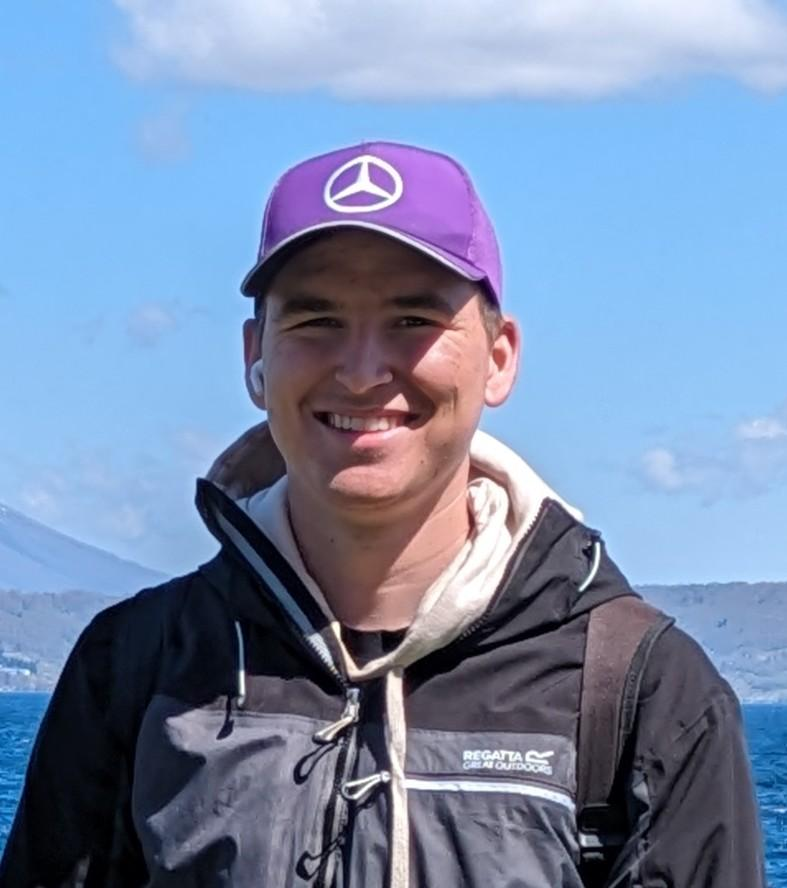
\includegraphics[width=2cm,valign=c]{images/Media.jpg}\\
		Abdul Mueed & Mechanical Engineering  & Theory & \includegraphics[width=2cm,valign=c]{images/image(1).jpg} \\ 
		Abdelrahman Shehata & Mechanical Engineering  & Discussion of results & 
\includegraphics[width=2cm,valign=c]{images/Image.jpg}\\
		Naim Alrifai & Mechanical Engineering & Conclusion & 
\includegraphics[width=2cm,valign=c]{images/Image(9).jpeg} \\\hline
		Munachi J Atuegbu & Mechanical Engineering & Last seen 11/29/24 & 
\includegraphics[width=2cm,valign=c]{images/profile.png} \\\hline
		Ehsan Haque & Mechanical Engineering & Approved Mitigation  & 
\includegraphics[width=2cm,valign=c]{images/profile.png} \\
	\end{tblr}
		\vspace*{\fill}
	
	\normalsize
	\newpage\newgeometry{top=0.2in,bottom=0.6in,left=0.8in,right=0.8in}
	\noindent\vspace{3em}
	\begin{center}
		\LARGE \textbf{Table of Contents}\\[-7em]
	\end{center}
	{
		\hypersetup{linkcolor=black}
		\tableofcontents
	}    
	
	
	\large\newpage\restoregeometry\vspace*{-20pt}
	
	\noindent
	
	\section{Abstract}
	In this experiment, we calibrated and compared the performance of multiple pressure-measuring devices, including two Bourdon gauges, a Budenberg pressure gauge, and a Hg glass manometer, using a reference pressure calibrator (DPI-603 Portable Pressure Calibrator). This device served both as the baseline for pressure measurements and as the source of the applied pressure, allowing us to apply both positive and negative pressures in increments of approximately 5 kPa. Through this process, we were able to get an thorough dataset that demonstrated notable differences in the pressure-measuring devices' performances. Our results revealed significant performance variations, with the Budenberg gauge showing exceptional accuracy (±0.59\% error) comparable to the Hg manometer (±0.58\%), while the Bourdon gauges exhibited larger errors (up to -47.59\% under vacuum conditions). These results highlighted the importance of selecting appropriate devices based on precision requirements and operating conditions, as well as the potential impact of human error in reading analog instruments like the Bourdon gauges.

	
	\newpage\vspace*{-20pt}

	\section{Introduction}
	In engineering and scientific applications, pressure measurement is essential, playing a critical role in fields such as fluid dynamics, meteorology, and industrial control. Over time, pressure-measuring instruments have evolved, from early liquid column manometers to modern mechanical and digital gauges, each designed to provide accurate measurements under varying conditions.\\[8pt]
	A key distinction in pressure measurement is between \textbf{absolute} and \textbf{gauge} pressure.\\ 
	Absolute pressure is measured relative to a vacuum, while gauge pressure is measured relative to atmospheric pressure. This distinction influences the design and function of pressure-measuring devices.\\[8pt]
	Historically, the invention of the Bourdon gauge by Eugène Bourdon in 1849 marked a significant advancement in pressure measurement. It provided a robust and reliable means of monitoring pressure in industrial settings, where durability and consistency were paramount.\\[8pt] 
	On the other hand, liquid column manometers, particularly those using mercury, have been essential in laboratory settings due to their precision in measuring small pressure differences.\\[1em]
	Despite the advantages of different pressure-measuring devices, each has limitations, such as calibration errors and environmental influences.\\[8pt]
	Previous studies have highlighted various challenges and findings related to pressure measurement devices. For example, a study by Hodgkinson et al. (2020) found that the accuracy of home blood pressure monitors varied significantly, with validated monitors showing a higher pass rate in static pressure tests compared to unvalidated ones. This emphasizes the importance of validation and calibration in ensuring the accuracy of pressure-measuring devices.\\[8pt]
	In this experiment, we aimed to evaluate the performance and accuracy of various pressure-measuring devices under controlled conditions, comparing their responses to varying pressure levels.
	
	\newpage\newgeometry{left=0.8in,right=0.8in,top=1in,bottom=0.7in}

	\section{Theory}

When discussing pressure, the primary consideration is its physical definition. It is fundamentally characterized as the force exerted per unit area on a surface, leading to effects such as deformation or displacement (measurable depending on the material and conditions of application). It as defined as:\vspace{-0.5em}
\begin{center}
	\begin{minipage}{0.51\textwidth}
		\centering
			\begin{equation}
				P = \frac{F}{A}
				\label{eq:pressure}
			\end{equation}
		\hspace*{2em}\wm{0.9}{
			\begin{itemize}[itemsep=-1mm]
				\item \( P \) : Pressure (Pa, Pascal)
				\item \( F \) : Force applied (N, Newton)
				\item \( A \) : Surface area (m\(^2\))
			\end{itemize}
		}\\[9pt]
		Average pressure $\left(P\right)$ assumes uniform distribution.\\[8pt]
		\begin{minipage}{0.45\textwidth}\centering
			Local pressure \( P_{\text{local}}\) varies spatially:
		\end{minipage}
		\begin{minipage}{0.45\textwidth}\vspace{-1em}
		\begin{equation}
			P_{\text{local}} = \frac{dF}{dA}
			\label{eq:localpressure}
		\end{equation}		
		\end{minipage}\\[8pt]\raggedright
		It peaks under concentrated loads (red zone) and vanishes at free edges (blue zone) revealing real-world stress hotspots (Figure \ref{fig:pressure}).
	\end{minipage}
	\hfill
	\begin{minipage}{0.46\textwidth}
		\vspace{-1.2em}\centering\hspace*{2.5em}
		\begin{tikzpicture}[scale=2,transform shape]
			\coordinate (c1) at (1,0,1);
			\coordinate (c2) at (-1,0,1);
			\coordinate (c3) at (-1,0,-1);
			\coordinate (c4) at (1,0,-1);
			\fill[blue!70!black,opacity=0.3] (c1) -- (c2) -- (c3) -- (c4) -- cycle;
			\begin{scope}
				\clip (c1) -- (c2) -- (c3) -- (c4) -- cycle;
				\begin{scope}[canvas is xz plane at y=0]
					\shade[inner color=red, outer color=blue!70!black, shading=radial,opacity=0.3] 
					(0,0) circle (1.36cm);
					\shade[inner color=red, outer color=blue!70!black!50!white, shading=radial, opacity=0.3] 
					(0,0) circle (1.2cm);
				\end{scope}
			\end{scope}
			\draw[thick] (c1) -- (c2) -- (c3) -- (c4) -- cycle;
			\draw[thick,-{Latex[scale=1.5,length=2mm,width=2mm]},line width=0.1mm] (0,1,0) node[above,right=1] {\large $\vec{F}$} -- (0,0,0);
			\draw[thick,<->] (1.05,-0.05,1.05) -- (-1.05,-0.05,1.05) node[midway,below=1.1] {\tiny$L_x$};
			\draw[thick,<->] (1.05,-0.05,1.05) -- (1.05,-0.05,-1.05) node[midway,right=1.1] {\tiny$L_x$};
			\node at (1.05,-0.05,1.05) [below] {$A$};
		\end{tikzpicture}
		\vspace{-1em}
		\captionof{figure}{Illustration of pressure application}
		\label{fig:pressure}
\end{minipage}\end{center}\vspace{-1.5em}
\subsection{Atmospheric Pressure}
Atmospheric pressure ($P_{\text{atm}}$) is the pressure exerted by the weight of air in the Earth's atmosphere. At sea level, it is approximately:
\begin{equation*}
	P_{\text{atm}} \approx 101.325 \text{ kPa} = 1 \text{ atm}
\end{equation*}
It decreases with altitude due to a reduction in air density, (See section \ref{Pressure Units} for more detail on the unit)\\[-1em]
\vspace{0.7em}\hrule\vspace{0.7em}\noindent
Atmospheric Pressure serves as the reference for gauge pressure, which is defined as:
\begin{equation}
	P_{\text{gauge}} = P_{\text{absolute}} - P_{\text{atm}}
\end{equation}
Thus, absolute pressure can be expressed as:
\begin{equation}
	P_{\text{absolute}} = P_{\text{gauge}} + P_{\text{atm}}
	\label{eq:absolute}
\end{equation}
Key pressure classifications include:\\
\vspace{-1em}
\begin{itemize}
	\item \textbf{Positive (or Gauge) Pressure ($P_{\text{gauge}} > 0$)}: Any pressure higher than local atmospheric pressure.
	\item \textbf{Negative (or Vacuum) Pressure ($P_{\text{gauge}} < 0$)}: Any pressure lower than atmospheric pressure but not reaching absolute zero.
\end{itemize}
\begin{center}\vspace{-1.5em}
\begin{formal}[(Farbod Tabesh, 2019)]{black!60!white}{white}\vspace{-0.7em}
\begin{minipage}[t]{0.48\textwidth}
	\subsection{Absolute Pressure}
	Absolute pressure is measured relative to a perfect vacuum, where no molecules exert force. It represents the total pressure exerted, including atmospheric pressure. In practical applications, absolute zero pressure is unattainable, but it serves as the theoretical baseline for all pressure measurements.
\end{minipage}\hfill
\begin{minipage}[t]{0.47\textwidth}
	\subsection{Gauge Pressure}
	Gauge pressure, also referred to as relative pressure, is measured with respect to local atmospheric pressure. Since atmospheric pressure varies with altitude and weather conditions, gauge pressure is useful for measuring pressure differences in industrial and scientific applications. It can be positive or negative, depending on whether the measured pressure is above or below atmospheric pressure.
\end{minipage}\\
\end{formal}
\end{center}

\vspace{-2em}
\newpage\noindent
\textbf{Vacuum Pressure Relation:}  
Any pressure below atmospheric pressure but above absolute zero pressure. Vacuum pressure is often measured as a positive value but represents a pressure below atmospheric pressure:
\begin{equation}
	P_{\text{vac}} = P_{\text{atm}} - P_{\text{absolute}}
\end{equation}
where higher vacuum pressure indicates a lower absolute pressure.\\[-1em]
\vspace{0.7em}\hrule\vspace{0.7em}\noindent
The following diagram illustrates all these pressure definitions more clearly.\\\vspace{-1em}
\begin{center}
\begin{tikzpicture}[scale=2,transform shape]	
	\def\floorx{5.5+2.5}
	\def\lapx{2.6+1.8}
	\def\twox{2.8+2}
	\def\onex{\floorx-0.4}
	
	\def\floory{-0.1}    
	\def\lapy{3+1}
	\def\twoy{0.5*\lapy}
	\def\oney{1.65*\lapy+0.5}
	
	\def\padding{0.7}
	
	\fill[bottom color=white, top color=gray] (0,0) rectangle (\floorx,\floory-0.08);
	\draw[-,gray!80!black] (0,0) -- (\floorx,0);    
	
	\fill[bottom color=white, top color=blue!50!white] (0,\lapy) rectangle (\lapx,\lapy-0.15);
	\draw[-,blue!50!white] (0,\lapy) -- (\lapx,\lapy);    
	
	\draw[-{Latex[scale=1.5,length=2mm,width=2mm]}] (\lapx-0.2,\lapy) -- (\lapx-0.2,\twoy) node[midway,fill=white, inner sep=2pt, text=black] {\tiny\wm{0.1}{\textsf{Rel. Press.\\ of point 2}}};    
	\draw[-{Latex[scale=1.5,length=2mm,width=2mm]}] (\lapx-0.2,0) -- (\lapx-0.2,\twoy) node[midway,fill=white, inner sep=2pt, text=black] {\tiny\wm{0.1}{\textsf{Abs. Press.\\ of point 2}}};
	
	\draw[-] (\lapx-0.4,\twoy) -- (\twox+\padding,\twoy);
	
	\draw[{Latex[scale=1.5,length=2mm,width=2mm]}-{Latex[scale=1.5,length=2mm,width=2mm]}] (\twox+\padding,\twoy) -- (\twox+\padding,\oney) node[midway,fill=white, inner sep=2pt, text=black] {\tiny\wm{0.2}{\textsf{Differential. Press.\\ Between 1 \& 2}}};
	
	\node[circle,draw=black, fill=orange, inner sep=0pt,minimum size=7pt] (b) at (\twox,\twoy) {};
	\node[above=1.4] at (\twox,\twoy) {\footnotesize \textsf{2}};
	
	\draw[-] (\onex,\oney) -- (\lapx-1,\oney);
	\node[circle,draw=black, fill=green, inner sep=0pt,minimum size=7pt] (a) at (\onex,\oney) {};
	\node[above=1.4] at (\onex,\oney) {\footnotesize \textsf{1}};  
	\draw[{Latex[scale=1.5,length=2mm,width=2mm]}-] (\lapx-0.6,\oney) -- (\lapx-0.6,\lapy) node[midway,fill=white, inner sep=2pt, text=black] {\tiny\wm{0.1}{\textsf{Rel. Press.\\ of point 2}}};   
	
	\draw[-{Latex[scale=1.5,length=2mm,width=2mm]}] (\onex*2.4,0) -- (\onex*2.4,\oney) node[midway,fill=white, inner sep=2pt, text=black] {\tiny\wm{0.1}{\textsf{Abs. Press.\\ of point 1}}};
	
	\node[right] at (0,\lapy-0.4) {\footnotesize \textcolor{blue!70!white}{\textsf{Local Atmospheric Pressure}}};
	
	\node[right] at (0,\lapy*2.4) {\scriptsize\wm{0.2}{\textsf{Positive\\ Pressure}}};
	\node[right] at (0,\lapy-\lapy) {\scriptsize\wm{0.2}{\textsf{Negative\\ Pressure\\ (Vacuum)}}};
	\node[left=-0.2cm] at (\floorx*0.5,-0.5) {\wm{0.3}{\scriptsize\textsf{Absolute Zero Pressure}}};
\end{tikzpicture}
\captionof{figure}{Representation of Pressures (Farbod Tabesh, 2019)}\label{representation of pressure}
\end{center}
\subsection{Differential pressure}
Differential pressure is the difference between the values of the pressures at different locations (Renke, 2024). For example, if the pressure at point 1 is $P_1$ and the pressure at point 2 is $P_2$, then the pressure difference from 1 to 2 is: 
\begin{equation}
	\Delta P=P_1-P_2
\end{equation}
\newpage
\subsection{Devices and Mechanisms}
\begin{formal}[(Brannan, n.d.)(InstTools, 2017)(ScienceDirect,n.d.)]{black!60!white}{white}
\vspace{-1em}
\subsubsection{Bourdon Gauges}	
A Bourdon gauge consists of a curled up tube, with one end closed and the other open to the system.\\[8pt] 
As the pressure increases, the tube uncurls which can then be used to give a reading of pressure. The tube has been flattened, which causes the pressure exerted outwards to act on two opposing flat planes, making the tube straighten in a more predictable fashion.\\[8pt]
The tip of the tube is connected to a linkage and a pivot, which is then connected to a movement (gearing system).\\[8pt]
This mechanism measures the mechanical movement of the tube resulting from the force created by the pressure. As shown in Equation \ref{eq:pressure}, if the area remains constant, force and pressure are directly proportional. This means that with knowledge of the mechanical properties of the tube material and the force required to move it, you can accurately determine the fluid pressure in the tube.\\[8pt] 
However, this requires the pressure to remain within certain boundaries. Excessive pressure could exceed the material's yield point, causing plastic deformation that would permanently damage the gauge and render it inaccurate.\\\vspace{-2em}
\paragraph{Types of Bourdon Gauges}\mbox{}\\[8pt]
There are three main types of Bourdon gauges, each with different sensitivities and pressure ratings:

\begin{itemize}
	\item \textbf{C-Type:}\\[8pt]
	\begin{minipage}{0.3\textwidth}\centering\hspace*{-1em}
		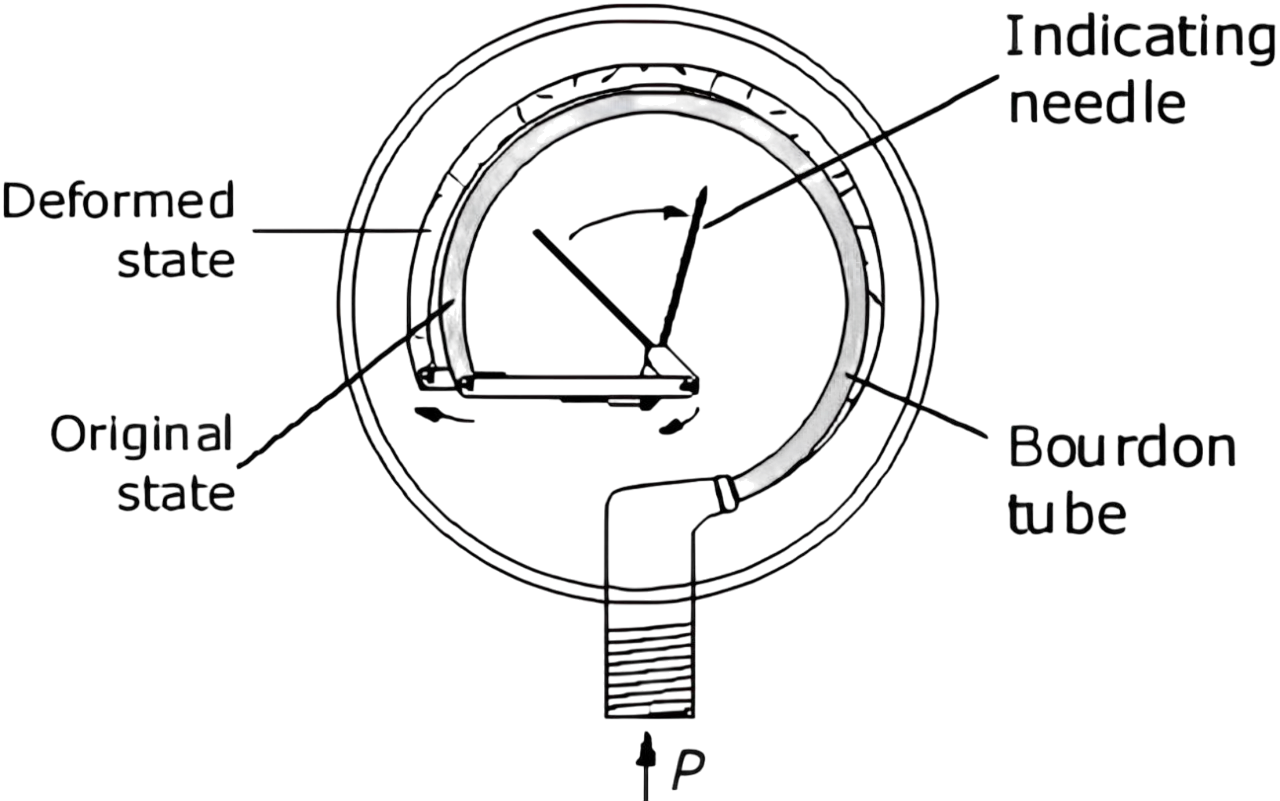
\includegraphics[width=1.1\textwidth]{images/ezgif-42a6b97cab4453(2)-Photoroom.png}
		\captionof{figure}{C-Type Bourdon gauge (Efunda, 2024)}
	\end{minipage}\hfill
	\begin{minipage}{0.6\textwidth}
		The C-Type Bourdon gauge features a flattened metal tube formed into a C-shape, with approximately 6mm of tip movement. This simple design makes it the \textbf{least accurate} Bourdon type, as the small movement requires mechanical amplification through gears and linkages.\\[5pt]
		These additional components can introduce inefficiencies and potential accuracy issues from loose or sticking parts.\\[5pt]
		Consequently, C-Type gauges are best suited for general-purpose applications where high precision isn't critical.
	\end{minipage}
   \item \textbf{Spiral:}\\[8pt]
	\begin{minipage}{0.3\textwidth}\centering
			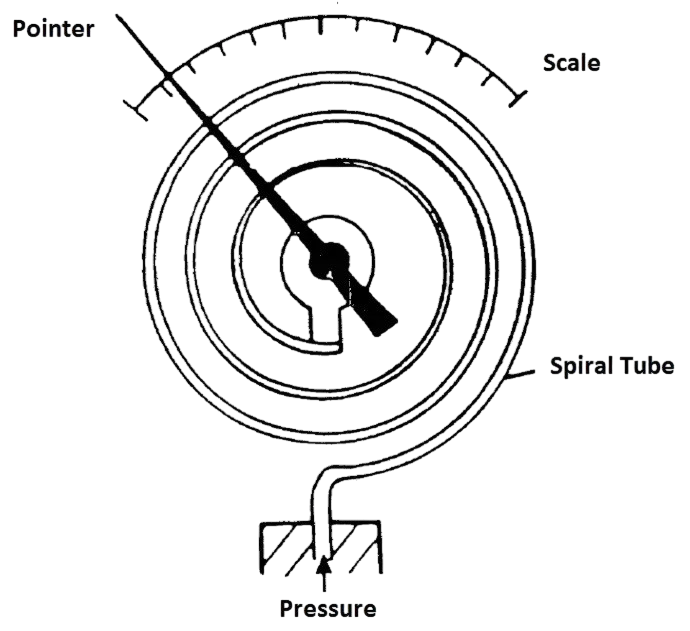
\includegraphics[width=1\textwidth]{images/ctype-ezgif.com-webp-to-jpg-converter-Photoroom.png}
			\captionof{figure}{Spiral Bourdon gauge (InstTools, 2017)}
	\end{minipage}\hfill
	\begin{minipage}{0.6\textwidth}
			This is similar to the C type bourdon gauge it follows the same principles of as pressure increases, it causes the coil to deform which can be measured and converted to a pressure reading.\\[5pt] Spiral gauges employ a coiled tube that provides 15-20mm of movement, three times more than C-types. This greater displacement eliminates the need for error-prone gear mechanisms.\\[8pt]
			The enhanced sensitivity ($\pm0.5\%$ accuracy) comes at higher cost, but proves essential for laboratory instruments and precision process control where small pressure changes matter.
	\end{minipage}\newpage
		
	\item \textbf{Helical:}
	\begin{figure}[H]
		\centering
		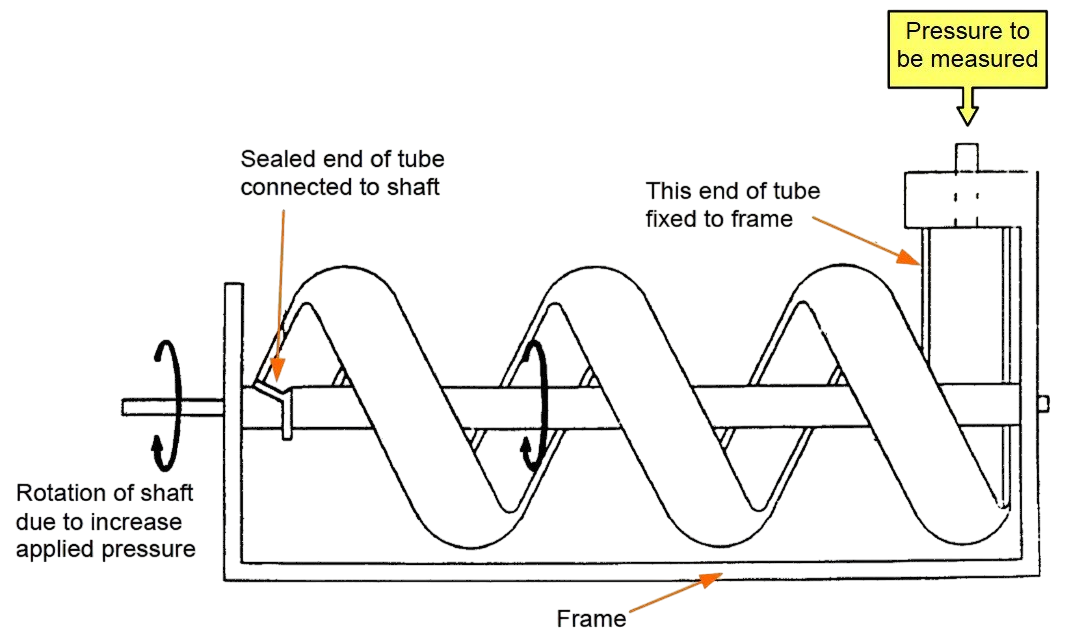
\includegraphics[width=0.5\textwidth]{images/helix-ezgif.com-webp-to-jpg-converter-Photoroom.png}
		\caption{Helical-type Bourdon gauge  (InstTools, 2017)}
		\label{fig:helical}
	\end{figure}

	The helical structure offers variable sensitivity across different pressure ranges. More coils enable operation at higher pressures while maintaining accuracy. The tip motion decreases as pressure increases, allowing customization of the optimal working range by adjusting the number of coils. Like spiral gauges, helical types maintain good efficiency due to minimal moving parts.
\end{itemize}
\end{formal}

\vspace{1em}
\subsubsection{Manometers}	

Manometers operate on the fundamental principle of hydrostatic equilibrium, where a fluid column balances pressure differences through gravitational force. The governing equation derives from the Navier-Stokes equations under static conditions:
\begin{equation}
	\frac{dP}{dz} = -\rho g
\end{equation}
\noindent 
For incompressible fluids, this integrates to the basic manometric equation:
\begin{equation}
	\Delta P = \rho g \Delta h
	\label{pressure}
\end{equation}
\begin{center}
\hspace{10em}\wm{0.7}{\centering
	\begin{itemize}[itemsep=-1mm,leftmargin=0cm]
		\item $P$ : Pressure (pascal, \si{\Pa})  
		\item $\rho$ : Density (kilogram per cubic meter, \si{\kg\per\m\cubed})  
		\item $g$ : Gravitational acceleration (meter per second squared, \si{\m\per\s\squared})  
		\item $\Delta h$ : Height difference (meter, \si{\m})
	\end{itemize}}
\end{center}
Key assumptions in classical manometry:
\begin{enumerate}
	\item \textbf{Constant fluid density ($\bm{\rho}$)}: Assumed invariant (valid for liquids under moderate pressure conditions)
	\item \textbf{Uniform gravitational acceleration ($\bm{g}$)}: Taken as 9.81 m/s$^2$ (varies less than 0.5\% across Earth's surface)
	\item \textbf{Negligible capillary effects}: Valid for tube diameters $>$10 mm (for water at standard conditions)
	\item \textbf{Minimal temperature variations}: Density changes are small ($\sim$0.1\% per \textdegree C for water)
	\item \textbf{Zero velocity condition}: Fluid is assumed stationary in the reference frame
\end{enumerate}

\paragraph{Manometer Types}\mbox{}\\[1em]
\small\textbf{1. U-Tube Manometer (Pressure Measurement Cases)}\\[8pt] \large
\noindent The U-tube manometer measures gas pressure by observing the displacement of a manometric fluid (typically mercury due to its high density). The pressure is determined by the height difference $h$ between the fluid levels in the two arms. Three common configurations are:\\[3pt]
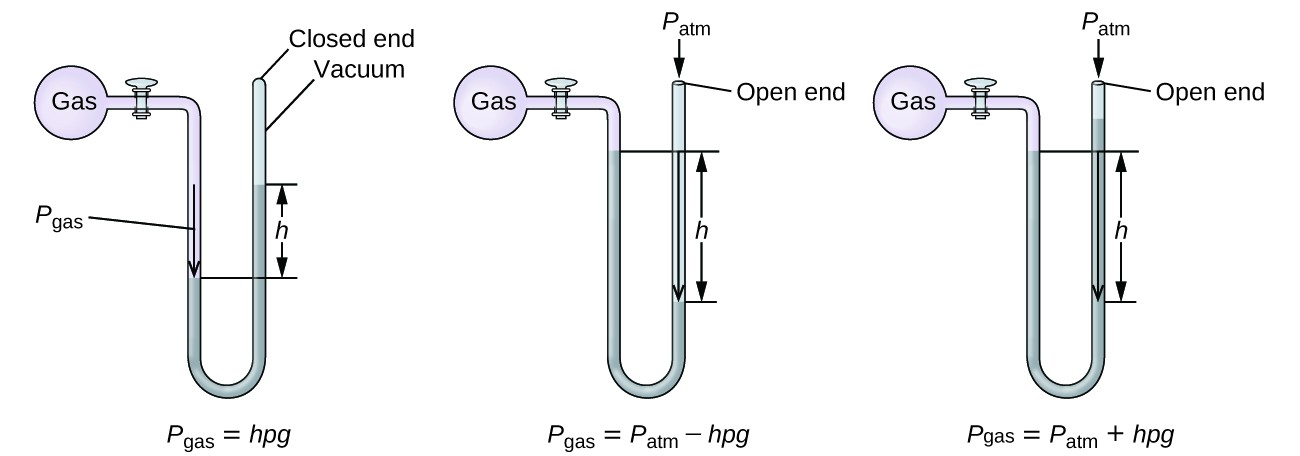
\includegraphics[width=1\textwidth]{images/CNX_Chem_09_01_Manometer1.jpg}
\captionof{figure}{U-Shaped Manometers  (LumenLearning, n.d.)}
\label{fig:cnxchem0901manometer1}
\vspace{1em}

\begin{center}
\begin{minipage}[t]{0.32\textwidth}
	\textbf{Closed-End:} \\
	The sealed arm serves as a vacuum reference ($P_2 = 0$), meaning the gas pressure is:
	\begin{equation}
		P_{\text{gas}} = \rho g h
	\end{equation}
\end{minipage}\hfill
\begin{minipage}[t]{0.32\textwidth}
	\textbf{Open-End:} \\
	Sub-atmospheric pressure\\ ($P_{\text{gas}}<P_{\text{atm}}$) causes downward displacement in the open arm:
	\begin{equation}
		P_{\text{gas}} = P_{\text{atm}} - \rho g h
	\end{equation}
\end{minipage}\hfill
\begin{minipage}[t]{0.32\textwidth}
	\textbf{Open-End:} \\
	For gas pressure above atmospheric ($P_{\text{gas}} > P_{\text{atm}}$), the manometer fluid rises in the open arm.	\begin{equation}
		P_{\text{gas}} = P_{\text{atm}} + \rho g h
	\end{equation}
\end{minipage}
\end{center}\vspace{0.3em}
For gases with negligible density ($\rho_f \ll \rho_m$), the fluid density $\rho$ simplifies to $\rho_m$ (e.g., mercury).\\[1em]
\begin{minipage}{0.5\textwidth}
	\small\textbf{2. Torricellian Barometer (Absolute Pressure)}\\[8pt]	
	\large The mercury barometer shows a basic measurement of atmospheric pressure.\\[8pt]
	The experiment uses a simple barometer to measure the pressure of air, filling it with mercury up until 75\% of the tube. Any air bubbles in the tube must be removed by inverting several times. After that, a clean mercury is filled once again until the tube is completely full. The barometer is then placed inverted on the dish full of mercury.  
\end{minipage}\hfill
\begin{minipage}{0.47\textwidth}\centering
	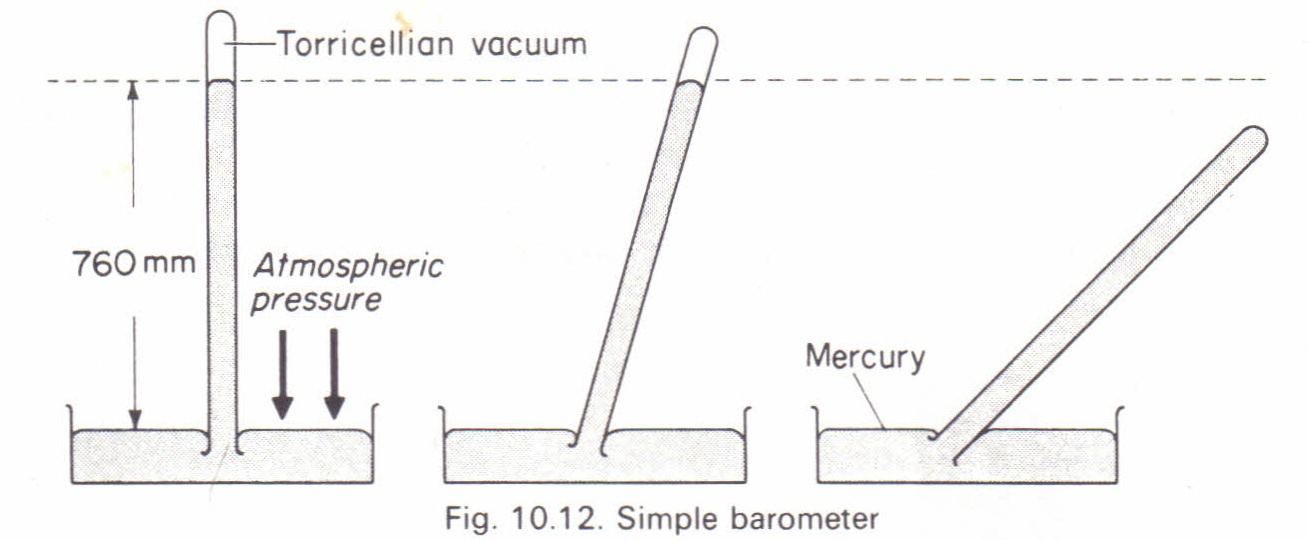
\includegraphics[width=1\textwidth]{images/1204.jpg}
	\captionof{figure}{Torricelli’s experiment. Simple barometer (PhysicMax, 2014)}
	\label{fig:1204}
\end{minipage}\\[6pt]
This causes the mercury in the tube to fall down until the difference between mercury on the surface and in the tube is about 760 mm. Even when the tube is shaken or tilted, the difference between the surface and in the tube is not affected due to the influence of atmospheric pressure. (Wikipedia, 2021)\\[6pt]
A notable function of the mercury barometer is the maintenance of an invention vacuum above the mercury column, where norm is essentially zero. The reason for mercury is its high density; mercury has a density of kg/m$^3$ at 20\textdegree C.

\newpage\newgeometry{left=0.8in,right=0.8in,top=1.23in,bottom=0.69in}

\subsection{Pressure Units}\label{Pressure Units}


\begin{center}
	\begin{tblr}{
			colspec={Q[2.3cm]Q[2.3cm]Q[2.3cm]Q[2.3cm]Q[2.3cm]Q[2.3cm]},
			hlines, vlines, 
			cells={valign=m, halign=c},
			rows={ht=2\baselineskip},
			row{1}={ht=2\baselineskip,
			font=\bfseries,bg=black!5!white},
			column{1}={font=\bfseries,bg=black!5!white}
		}
		\SetCell{bg=black!10!white,fg=black}\textbf{Unit} & \textbf{Pa} & \textbf{bar} & \textbf{psi} & \textbf{atm} & \textbf{cm Hg} \\
		Pa & 1& $1 \times 10^{-5}$ & $1.450 \times 10^{-4}$&$9.869 \times 10^{-6}$ & $0.00750062$ \\
		bar& $1 \times 10^{5}$ & 1& 14.5038& 0.986923    &75.0062 \\
		psi & 6894.76 & 0.0689476&1& 0.068046&51.7149 \\
		atm& 101325&1.01325&14.6959& 1 & 76.0032 \\ 
		cm Hg&1333.22&0.013332&0.19337& 0.013158 & 1 \\
	\end{tblr}
\end{center}	\vspace{-1em}\captionof{table}{Standard Pressure Unit Conversions}\label{table:Pressure_Unit_Conversions}


\tikzexternaldisable

\begin{briefillus}{Pascal}{}
	The Pascal (Pa) is the SI unit of pressure, named after the French mathematician and physicist Blaise Pascal. It is defined as one Newton per square meter (\si{\newton\per\square\meter}). 
	\[1\,\text{Pa}=1\,\text{kN}\ \text{m}^{-2}\]
	As a relatively small unit, the Pascal is commonly used in scientific fields such as laboratory research or atmospheric studies.
\end{briefillus}

\begin{briefillus}{Atmosphere}{}
	The atmosphere (atm) is a unit of pressure defined as the average atmospheric pressure at sea level on Earth. Were \[1\,\text{atm}\approx101\, 325\,\text{Pa}\]
	The atmosphere is commonly used in chemistry and physics to describe gas pressures, especially in contexts like gas laws (e.g., Boyle's Law and Charles's Law), as well as in scuba diving to describe underwater pressures. It is used for convenience, providing a standardized unit for atmospheric pressure in various scientific and engineering applications.
\end{briefillus}

\begin{briefillus}{Bar}{}
	The bar is a metric unit of pressure, though it is not part of the International System of Units (SI). It is defined as \[1\,\text{bar}=100\, 000\,\text{Pa}\] 
	This exact by definition. However, the relationship between bar and atm involves a small fractional difference due to the empirical value of standard atmospheric pressure, it is very close, specifically $$1\,\text{bar}\approx0.986923\,\text{atm}$$ Which is just 1.013\% off. The bar is commonly used in meteorology, engineering, and industrial applications, as it provides a convenient scale for measuring pressures near atmospheric pressure.
\end{briefillus}

\begin{briefillus}{Pound per square inch}{}
	The pound per square inch (psi) is a unit of pressure primarily used in the United States and other countries that follow the Imperial system. It is defined as the pressure exerted by one pound-force applied to an area of one square inch. PSI is widely used in automotive, mechanical engineering, and hydraulic systems, such as measuring tire pressure.\\[8pt]
	The conversion factor between psi and Pascal is given as:
	\[1 \, \text{psi} = 6894.76 \, \text{Pa}.\]
	This conversion is derived from the definition of the pound-force (lbf) and the inch.\\
	One \textbf{pound-force (lbf)} is defined as the force required to accelerate a mass of one pound under the influence of gravity. In the metric system, 1 pound-force is approximately equivalent to 4.44822 Newtons (N). This is based on the following formulation:
	\[1\,\text{lbf}=1\,\text{lb}\times g\]
	\[1 \, \text{lbf} = 0.453592 \, \text{kg} \times 9.80665 \, \text{m/s}^2 = 4.44822 \, \text{N}.\]
	The force of one pound-force is applied over an area of one square inch. One square inch is defined as:
	\[1 \, \text{inch}^2 = 0.00064516 \, \text{m}^2.\]
	Thus, the conversion from psi to Pascal is calculated by dividing the force in Newtons by the area in square meters:
	\[1 \, \text{psi} = \frac{4.44822 \, \text{N}}{0.00064516 \, \text{m}^2} \approx 6894.76 \, \text{Pa}.\]
	This precise conversion reflects the accurate definitions of the pound-force and the inch, with the result ensuring consistent and reliable unit conversion between the Imperial and SI systems.
\end{briefillus}
\begin{briefillus}{Millimeter of Mercury}{}
	The millimeter of mercury (mmHg) is a unit of pressure historically based on the height of a mercury column that exerts a given pressure. It is commonly used in medical and scientific applications, particularly in measuring blood pressure and vacuum pressures.\\[8pt]
	It is defined as:
	\[1\,\text{mmHg} = 133.322\,\text{Pa}\]
	\begin{minipage}{0.9\textwidth}		
		This conversion is derived from the hydrostatic pressure equation:\\
		\[P = \rho g h\]
		\begin{itemize}[itemsep=-1mm]
			\item \(\rho : \text{Density of mercury}\, (13.5951 \, \text{g/cm}^3)\)
			\item \(g : \text{Gravitational acceleration}\, (9.80665 \, \text{m/s}^2)\)
			\item \(h : \text{Height}\, (\text{mm},\, \text{interchangeable})\).	
		\end{itemize}
	\end{minipage}\hspace{-7em}
	\begin{minipage}{0.2\textwidth}\vspace{-2em}
		$$\frac{g}{cm^3} \times \frac{m}{s^2} \times mm$$
		$$g\frac{m}{s^2} \times\frac{mm}{cm^3}$$
		$$10^{-3}N \times10^{3}m^{-2}$$
		$$N m^{-2} = \text{Pa}$$
	\end{minipage}\\[8pt]
	Although mmHg is not an SI unit, it remains widely used in medicine (e.g., blood pressure readings of 120/80 mmHg) and laboratory sciences for its convenience in low-pressure measurements.
\end{briefillus}		\vspace*{\fill}\noindent\footnotesize{The \textbf{torr} (symbol: Torr) is a unit of pressure based on an absolute scale, defined as exactly 1/760 of a standard atmosphere (101325 Pa). Thus one torr is exactly 101325/760 pascals ($\approx$ 133.32 Pa) (Wikipedia, 2025). This is a redacted unit in the context of this study}
\tikzexternalenable

	
	\newpage\vspace*{-20pt}\large
	\section{Method \& Experimental Procedures}\label{Method_Experimental_Procedures}
	%We are first given a table to record our findings as shown:\footnote{We started of in the lab by doing the refrigerator but this is redacted as its not a part of this lab report, following this we did the pressure lab experiment.}
	\vspace*{\fill}
	\begin{figure}[H] 
			\centering 
		    \begin{tikzpicture}[auto,
			block/.style ={rectangle, draw=gray!70!black, thick, fill=white!94!black, text width=1em,align=center, rounded corners, minimum height=2em},
			block1/.style ={rectangle, draw=gray!70!black, thick, fill=white!94!black, text width=5em,align=center, rounded corners, minimum height=2em},
			line/.style ={draw, thick, -latex',shorten >=2pt},
			cloud/.style ={draw=red, thick, ellipse,fill=red!20,
				minimum height=1em}]
			\node[anchor=center] (image) at (-10,0) {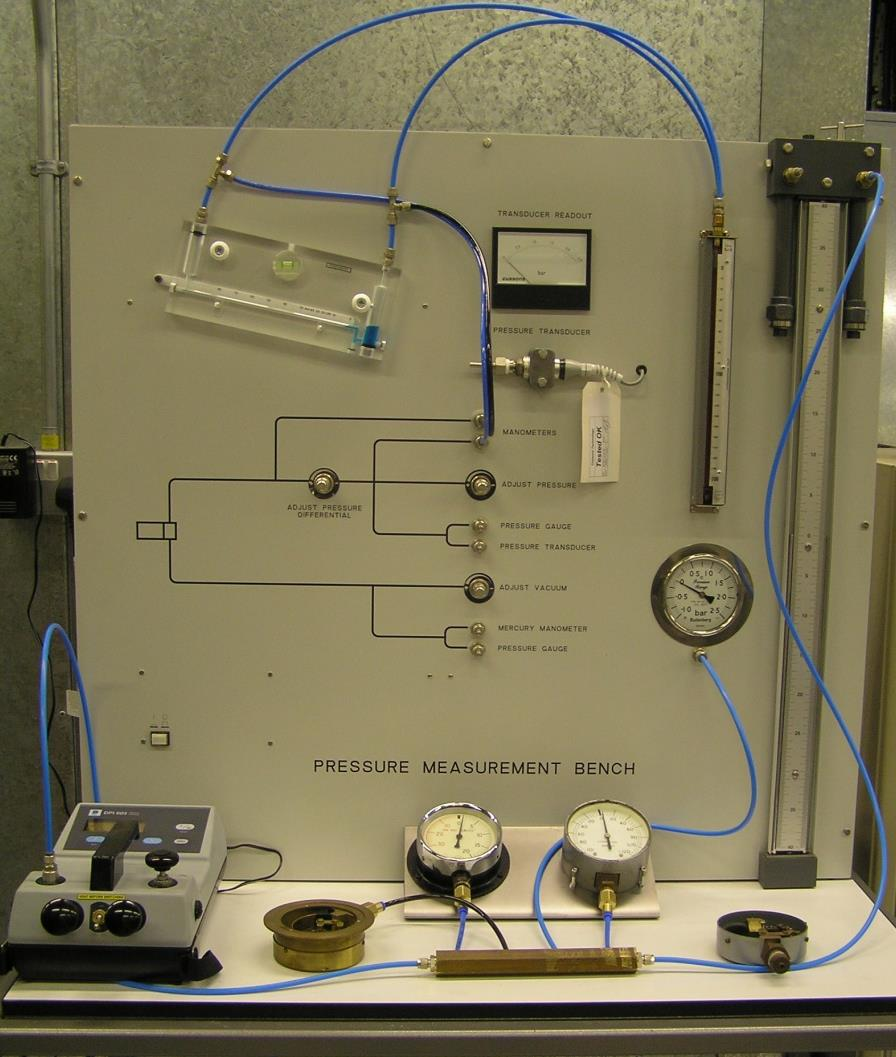
\includegraphics[width=0.9\textwidth]{extracted_images/image_7_1.png}};
			\node[block] (A) at (-9.85,-4.5) {1};
			\node[block] (B) at (-7.15,-4.5) {2};
			\node[block1] (Gauge) at (-8.5,-3.5) {Bourdon Gauge};
			%\draw[line] (Gauge.south) -- ++(0,-0.25) -| (A.north);
			%\draw[line] (Gauge.south) -- ++(0,-0.25) -| (B.north);			
			\node[block1] (Gauge) at (-15.5,-4.2) {Pressure calibrator};
			\node[block1] (Gauge) at (-7.5,-1.1) {Pressure Gauge};
			\node[block1] (Gauge) at (-3.5,7.6) {Mercury Glass Manometer};
		\end{tikzpicture}
		\caption{Pressure Measurement Bench} 
		\label{fig:pressure_measurement_bench} 
	\end{figure}
	\vspace*{\fill}
	\newpage
	
	\begin{figure}[H] 
			\centering 
			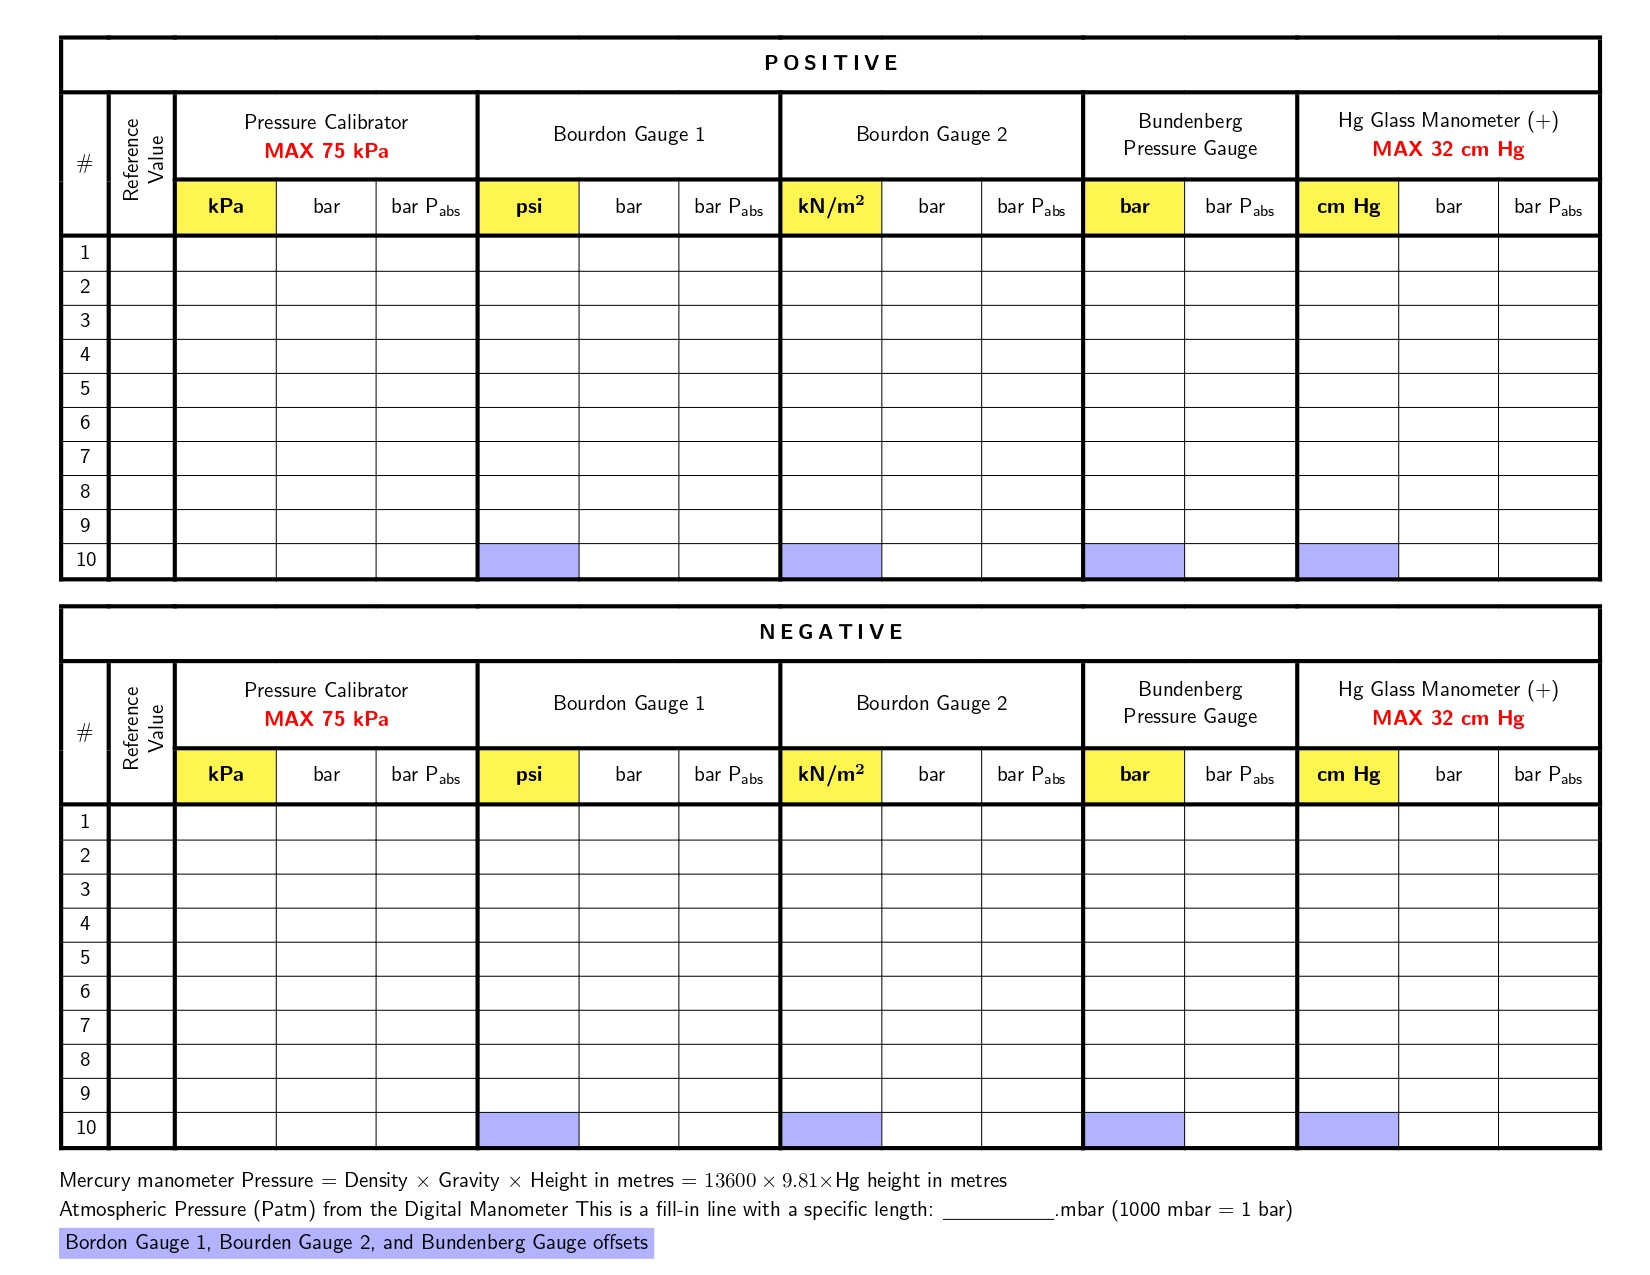
\includegraphics[width=1\textwidth,cfbox=gray!15 1pt]{images/tableland-1_page-0001.jpg} 
			\caption{Form for recording pressure measurements} 
			\label{fig:pressurestable} 
	\end{figure}
	\underline{The experiment \textbf{summary} reads:}\\[1em]
	The instructor has given a very elaborative demonstration about the functioning of pressure calibrator and has taken us through setting up the entire apparatus and interpreting the corresponding gauge readings.\\[1em]
	Before the onset of this experiment, safety drills were provided for everybody, including data compromising precautions and safety measures set for every participant involved in the experiment.\\[1em]
	The gauge readings and pressures applied at very subtle levels were evaluated in a collaborative effort to obtain a consensus upon acceptable values to be entered in the predefined pressure measurement table (see Figure \ref{fig:pressurestable}).\\[1em]
	The \textbf{exact steps} given to us are, in detail:


\newpage\newgeometry{left=0.8in,right=0.8in,top=1.1in,bottom=0.6in}
\begin{minipage}{0.52\textwidth}	
	\subsection{Operating Procedure}
	\begin{enumerate}[left=0in,itemsep=2mm]
	    \item The instructor inspected the test rig’s pneumatic connections to ensure they were secure.  
		\item The instrument’s vent valve was opened as part of the setup process.  
		\item Given the choice between vacuum (\textsf{\textcolor{blue}{-}}) and excess (\textsf{\textcolor{red}{+}}) pressurized, we initially set the selector on the front of the DPI-603 ($\pm$VE in Figure \ref{fig:DPI-603}) to positive pressure. This setting allowed us to apply the necessary excess pressure for the procedure.  
		\item The unit was powered on by pressing the power button.  
		\item Using the pressure units button, we cycled through the available options (in Hg, bar, etc.) and selected kPa.  
	\end{enumerate}
\end{minipage}\hspace{1em}
\begin{minipage}{0.45\textwidth}
	\begin{figure}[H] 
		\centering 		
		\begin{tikzpicture}[scale=0.45,transform shape]
			\node[anchor=center] (image) at (0,0) {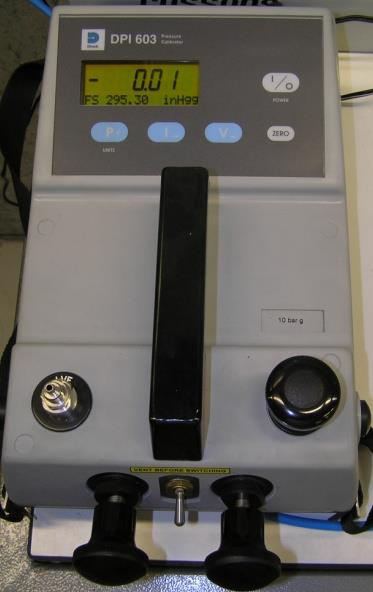
\includegraphics[width=1\textwidth]{extracted_images/image_8_1.png}};
     \draw[{Latex[length=3mm,width=3mm]}-,line width=0.5mm] (3.2, -2.2) -- (5, -3) node[above=1mm,right] {\Huge Vent Valve}; 
		
		    \draw[{Latex[length=3mm,width=3mm]}-,line width=0.5mm] (-2, 3.4) -- (-5, 3) node[left=14mm,below=-10mm] {\Huge \wm{1}{Pressure\\ Units}}; 
		
		\draw[{Latex[length=3mm,width=3mm]}-,line width=0.5mm] (-0.15, -5) -- (-0.15, -8) node[below=1mm] {\Huge $\pm \text{VE}$}; 
		
		\draw[{Latex[length=3mm,width=3mm]}-,line width=0.5mm] (1.35, -6.3) -- (3, -8) node[below=6.5mm,right] {\Huge\text{Hand Pump}}; 
		
		\draw[{Latex[length=3mm,width=3mm]}-,line width=0.5mm] (1.35-3, -6.3) -- (-3, -8) node[below=5.9mm,left] {\Huge\text{Volume Control}}; 
		
		\draw[{Latex[length=3mm,width=3mm]}-,line width=0.5mm] (-1.5, 5) -- (-3.5, 7.4) node[above=5.9mm,left=-1cm] {\Huge\text{Main Display}}; 
		
		\draw[{Latex[length=3mm,width=3mm]}-,line width=0.5mm,draw=black] (2.5, 5) -- (4.3, 7.4) node[above=5.9mm,right=-1cm] {\Huge\text{Power}}; 		
		\end{tikzpicture}
		\caption{DPI-603 Portable Pressure Calibrator} 
		\label{fig:DPI-603} 
	\end{figure}
\end{minipage}\\[0pt]\noindent
\begin{enumerate}[left=0in]
\item[6.] The vent valve was closed and used to zero the instrument. It was concluded that this procedure should be carried out by the instructor due to the vent valve’s sensitivity.  
\end{enumerate}\vspace{0.6em}\noindent
Here Steps 1-6 primarily cover the setup phase and were mainly carried out by the instructor. It was now our role to conduct the rest of the experiment, which proceeded as follows:\\[-3pt]
\begin{enumerate}[left=0in]
\item[7.] We used the hand pump to pressurize the system to the required value. To achieve precise control, we vented air using the vent valve and adjusted the pressure by pumping air as needed.
\item[8.] Once the required incremental was observed on the pressure calibrator, we then observe and recorded the readings seen on the following gauges:\\[8pt]
\end{enumerate}
	\begin{minipage}{0.45\textwidth}
			\hspace{0.9em}\begin{minipage}{1\textwidth}\centering
			\begin{minipage}{0.45\textwidth}\centering
				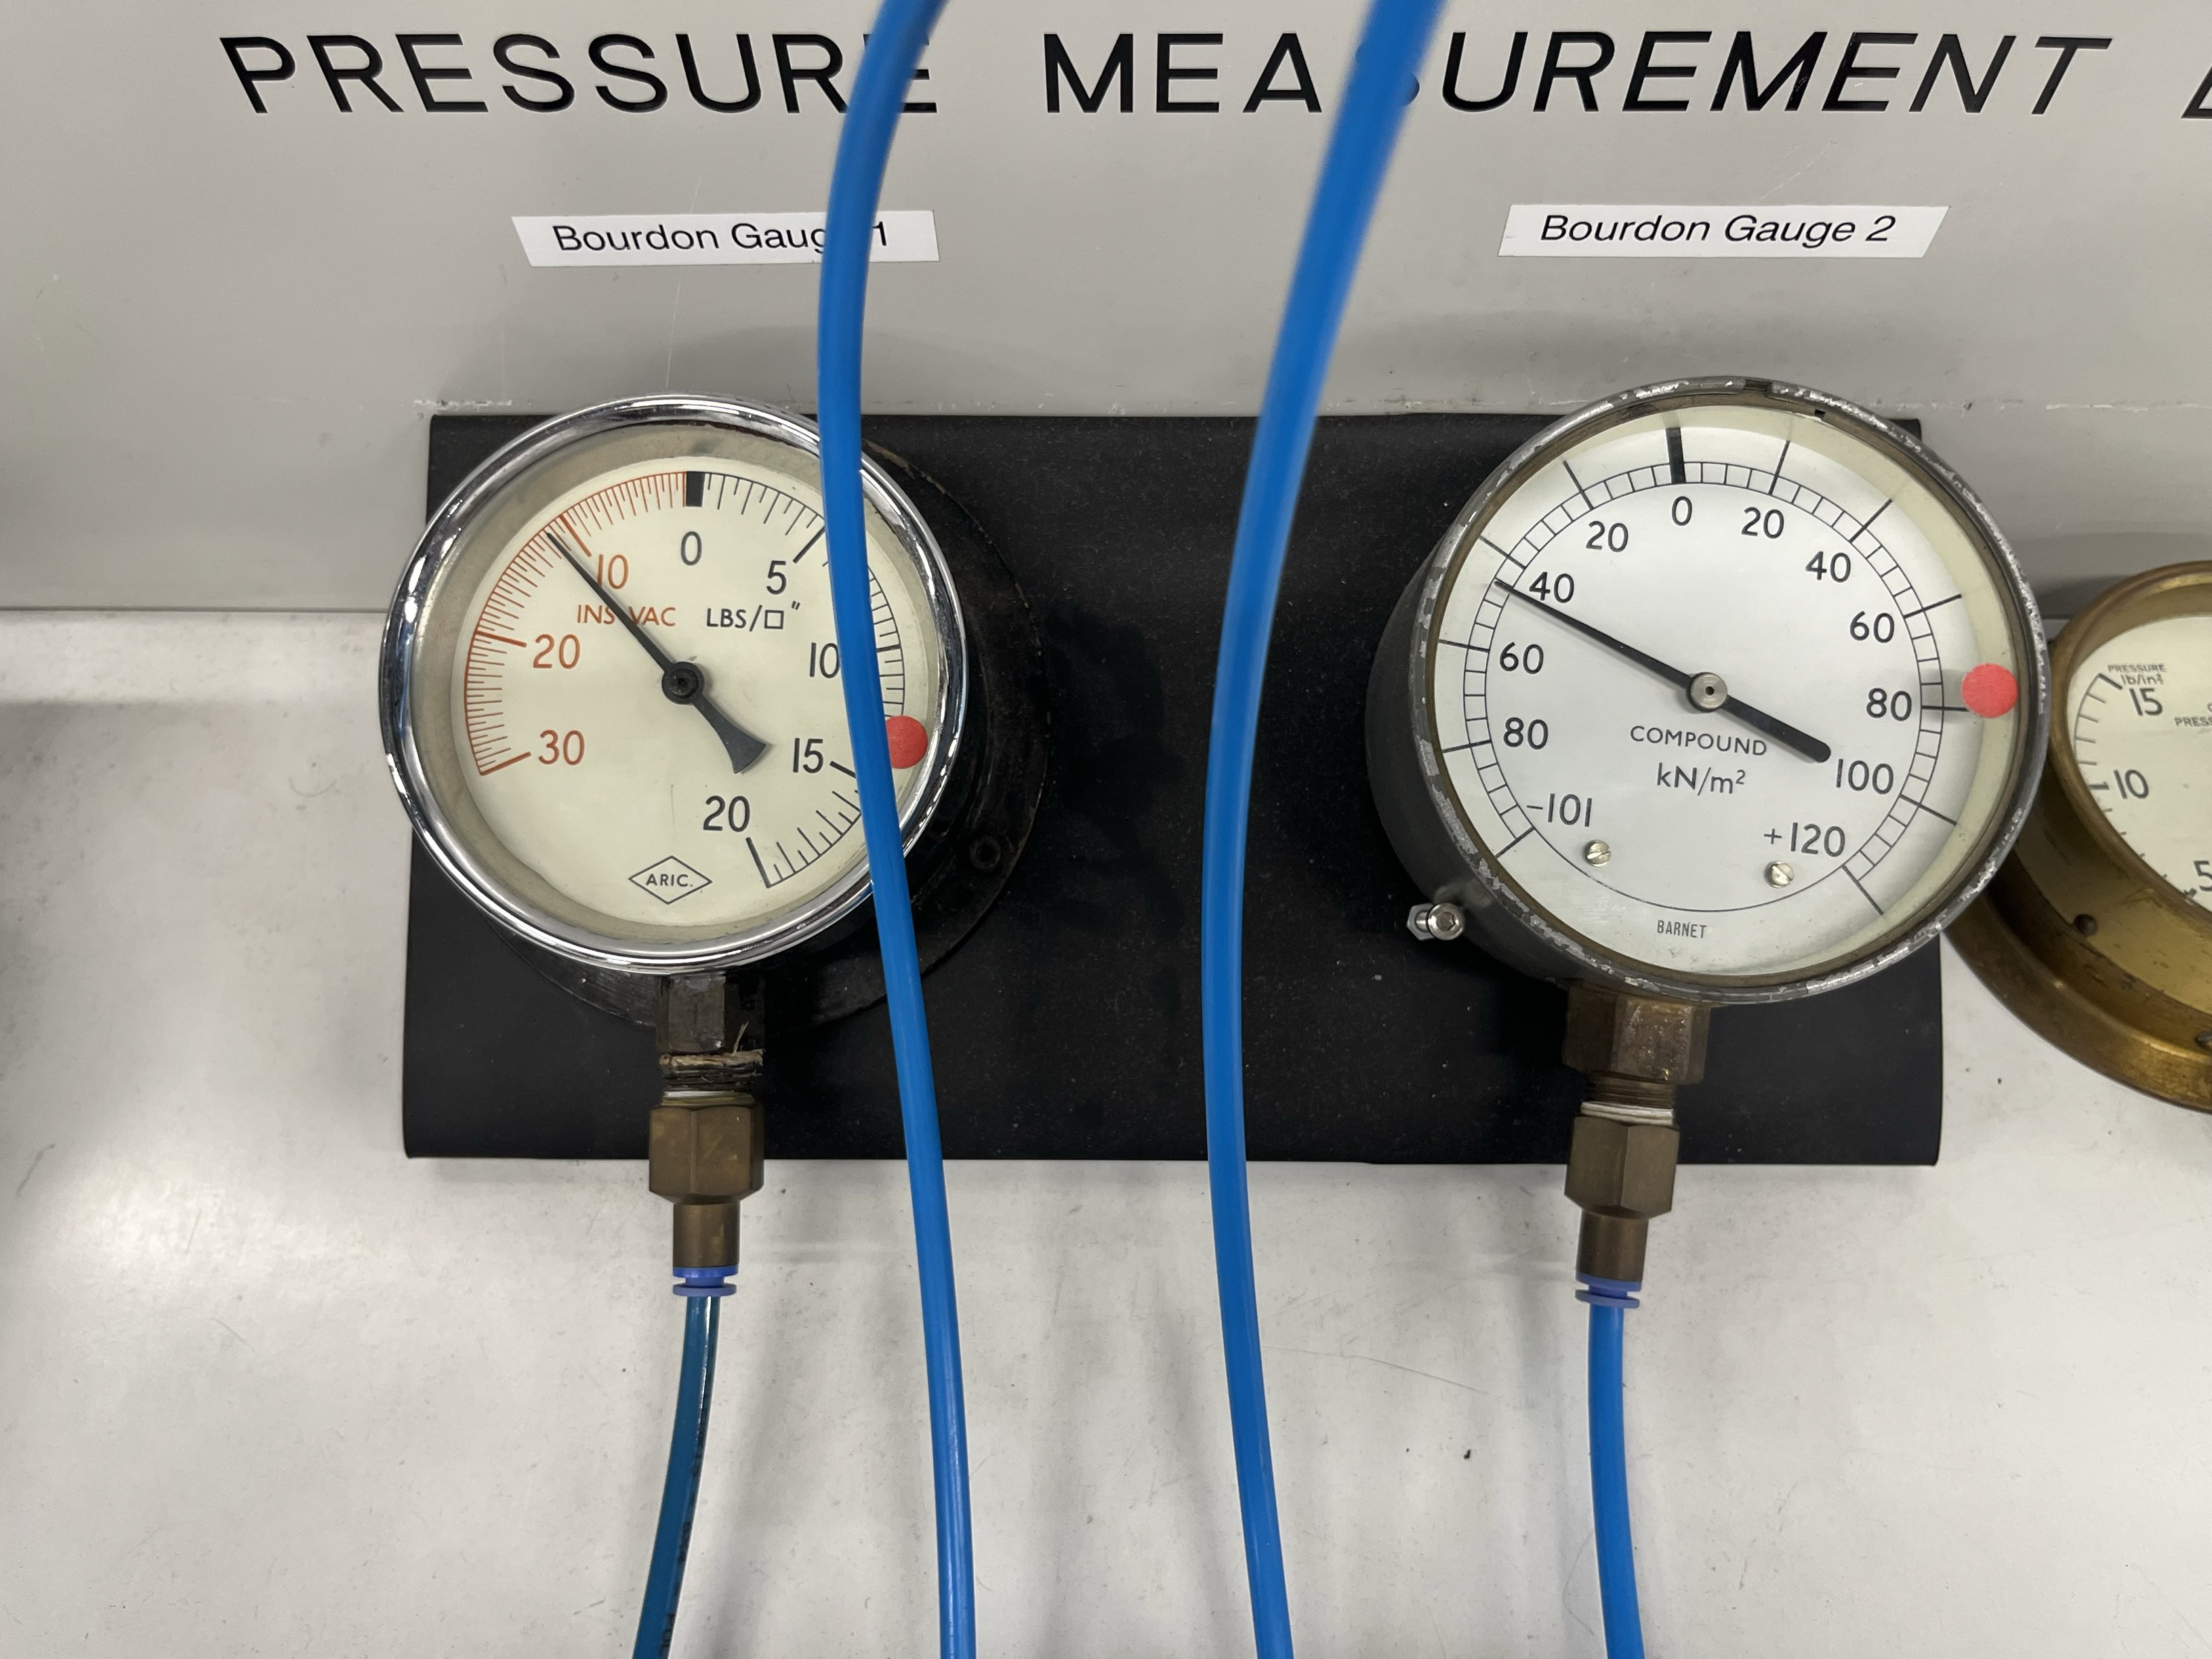
\includegraphics[width=1.2\textwidth]{images/Image(1)2.jpg}\\[0.5em]
				\rotatebox[origin=c]{0}{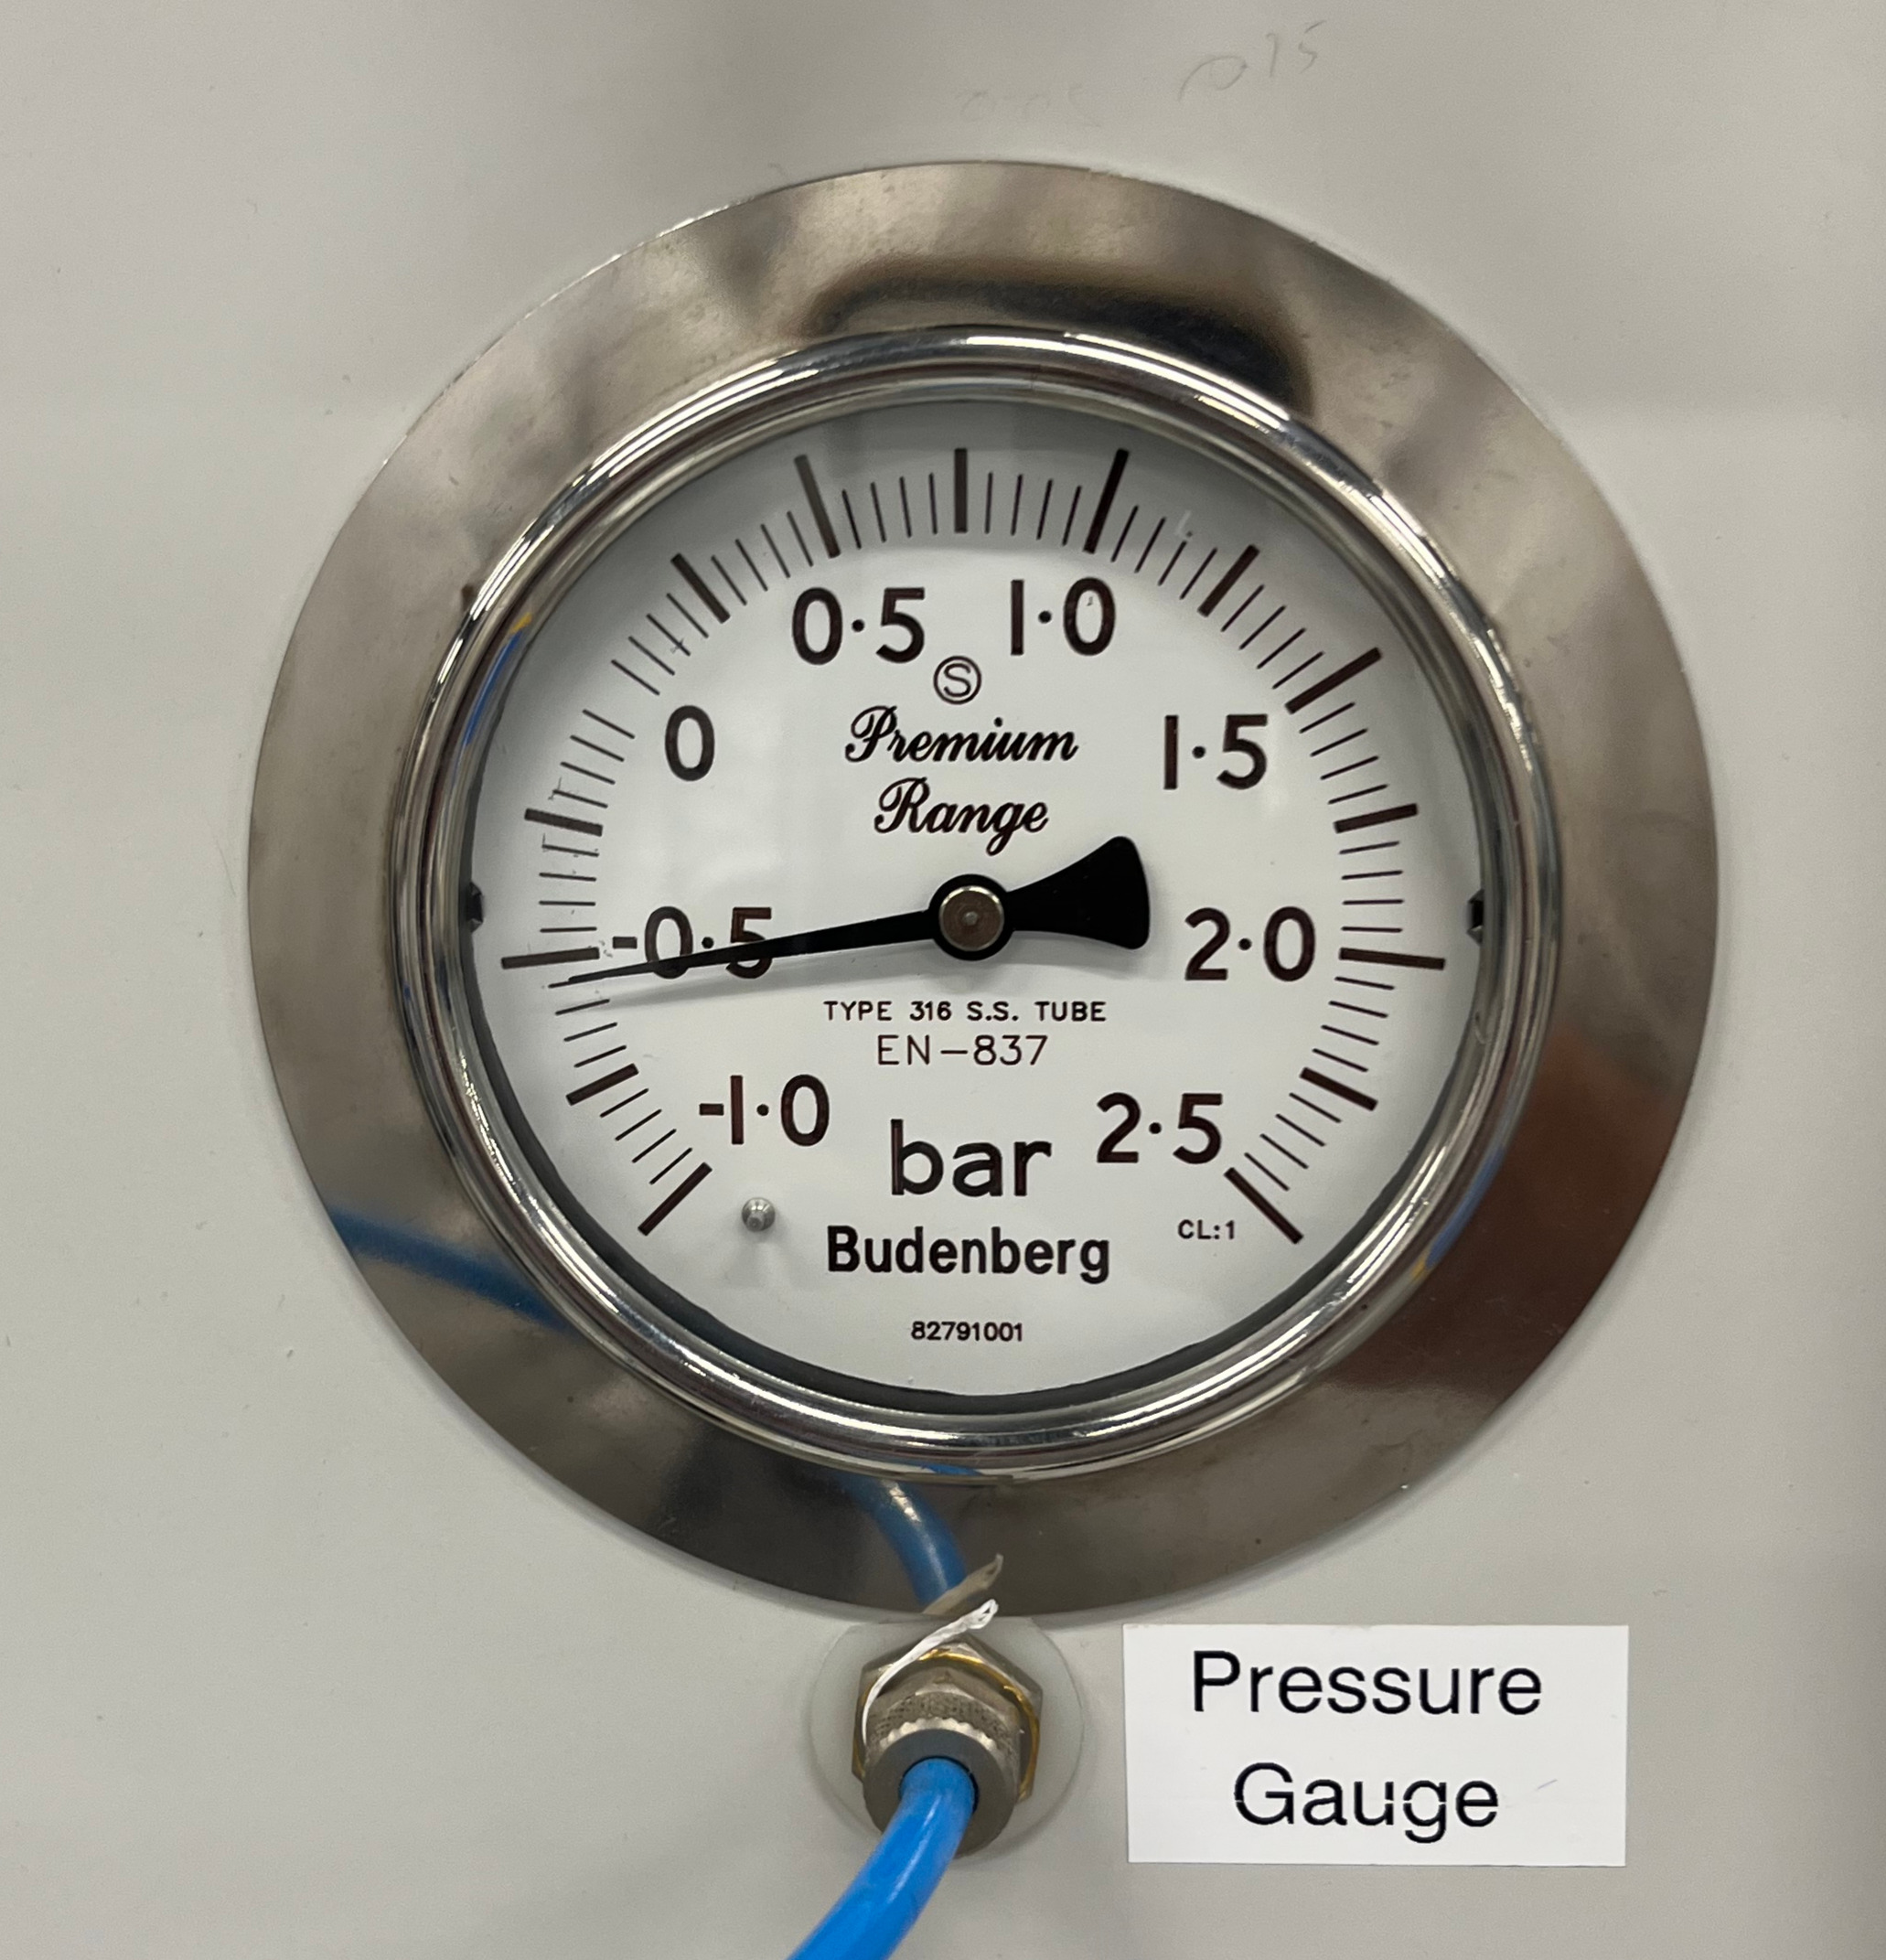
\includegraphics[width=1.2\textwidth]{images/Image(6).jpg}}
			\end{minipage}\hspace{0.5em}
			\begin{minipage}{0.4\textwidth}\centering
				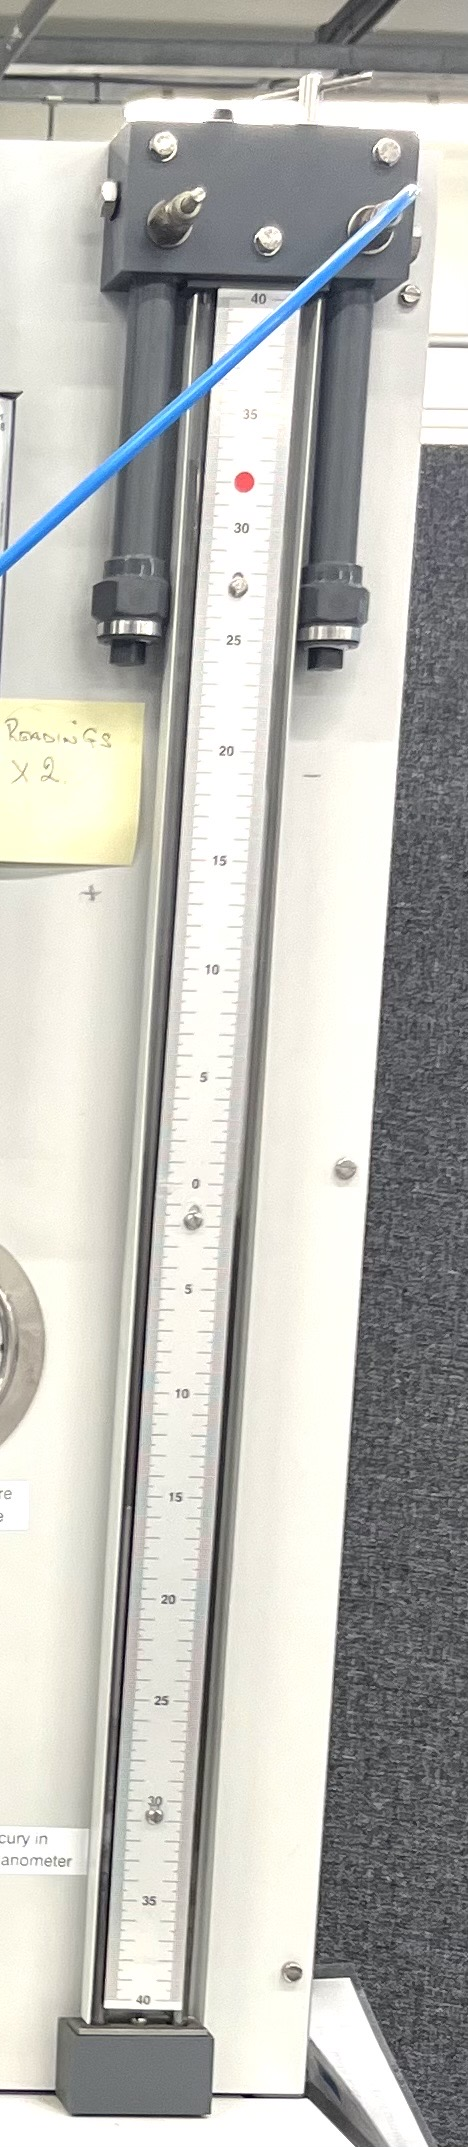
\includegraphics[width=0.55\textwidth]{images/Image(2).jpg}
			\end{minipage}
			\end{minipage}
			
			\centering
			\captionof{figure}{Gauges \& Manometer}\small Refer to Figure \ref{fig:pressure_measurement_bench} for illustrations labels.
	\end{minipage}
	\begin{minipage}{0.51\textwidth}\vspace{-2em}\raggedright
		\begin{enumerate}[left=0in]
			\item[9.]  By reaching on a agreement as a team over what is being read on the instruments for this related pressure value on the calibrator, we recorded them in the designated pressure measurement table (Figure \ref{fig:pressurestable}). 
			\item[10.] This procedure (Steps 7-9) is repeated, beginning with an \textbf{initial reading of 0 kPa} and continuing until the tenth increment, with each increment approximately $+5$ kPa.
			\item[11.] Once we're done, we go back and repeat steps 6–10, except this time we do for the vacuum ($-5$kPa).
		\end{enumerate}\noindent
		Could of been more detailed, but this will suffice, this concludes everything that was done in the lab so that we may draw conclusions from the information in the drawn tables.
	\end{minipage}
	

	\newpage\newgeometry{left=0.8in,right=0.8in,top=1in,bottom=0.5in}
	\section{Data, Calculations and Results}
	\tikzexternaldisable
	\subsection{Modifying the initial dataset}


	\hspace*{-2.2em}	
	\begin{minipage}{1.1\textwidth}
\begin{datasetbox}{Original Measurements}{data:orig}
	\begin{minipage}{0.23\textwidth}
		\begin{tcolorbox}[title={\color{black}\normalsize \textbf{Pressure Calibrator}}, colback=SkyBlue!6!white, 
			colframe=SteelBlue!30!white, boxrule=0.5mm, width=\textwidth]
		\hspace*{-0.82em}
		\begin{minipage}{1.2\textwidth}\centering
		\textbf{\textsf{kPa}}\\[8pt]
		\begin{tblr}{
					colspec={X[1cm]X[1cm]},
					hlines,vlines,
					cells={valign=m,halign=c,bg=white},
					rows={ht=1\baselineskip},
					row{1}={ht=1\baselineskip,font=\bfseries},
				}
				\Large\textsf{\textcolor{red}{+}}&\wm{0.2}{\vspace{0.1cm}\Large\textsf{\textcolor{blue}{-}}}\\\hline
				0  & 0  \\
				5.7  & -5.6  \\
				10.4 & -12.1 \\
				16.0 & -18.0 \\
				21.1 & -21.8 \\
				27.7 & -25.4 \\
				34.2 & -29.3 \\
				40.0 & -33.6 \\
				46.1 & -37.6 \\
				52.2 & -41.7 \\
			\end{tblr}
			\captionof{table}{Pressure Calibrator}
		\end{minipage}
		\end{tcolorbox}
	\end{minipage}
	\begin{minipage}{0.75\textwidth}
	\begin{tcolorbox}[
		title={\color{black}\normalsize \textbf{Pressure measuring instruments}},
		colback=MetallicSunburst!6!white, 
		colframe=ChineseGold!30!white, 
		boxrule=0.5mm, 
		width=1\textwidth
		]
		\begin{minipage}{1.03\textwidth}
			\hspace*{-1em}
			\centering	
			\begin{minipage}{0.225\textwidth}
			\centering
			\textbf{\textsf{psi}}\\[8pt]
			\begin{tblr}{
					colspec={X[1cm]X[1cm]},
					hlines,vlines,
					cells={valign=m,halign=c,bg=white},
					rows={ht=1\baselineskip},
					row{1}={ht=1\baselineskip,font=\bfseries},
				}
				\Large\textsf{\textcolor{red}{+}}&\wm{0.2}{\vspace{0.1cm}\Large\textsf{\textcolor{blue}{-}}}\\\hline
				1.0  & 1.2  \\
				2.0  & 0.4  \\
				2.6  & -0.5  \\
				3.4  & -2.0  \\
				4.1  & -2.8  \\
				5.0  & -4.0  \\
				6.0  & -6.0  \\
				6.8  & -7.1  \\
				7.6  & -8.3  \\
				8.5  & -9.5  \\
			\end{tblr}
			\captionof{table}{Bourdon Gauge 1}
		\end{minipage}
			\hfil
			\begin{minipage}{0.225\textwidth}
			\centering
			\textbf{\textsf{kN/m$\bm{^2}$}}\\[8pt]
			\begin{tblr}{
					colspec={X[1cm]X[1cm]},
					hlines,vlines,
					cells={valign=m,halign=c,bg=white},
					rows={ht=1\baselineskip},
					row{1}={ht=1\baselineskip,font=\bfseries},
				}
				\Large\textsf{\textcolor{red}{+}}&\wm{0.2}{\vspace{0.1cm}\Large\textsf{\textcolor{blue}{-}}}\\\hline
				1.0  & 2.5  \\
				8.0  & -1.0  \\
				14.0 & -9.0  \\
				20.0 & -15.0 \\
				25.0 & -20.0 \\
				30.0 & -23.0 \\
				39.0 & -27.0 \\
				45.0 & -32.0 \\
				50.0 & -36.0 \\
				57.0 & -40.0 \\
			\end{tblr}
			\captionof{table}{Bourdon Gauge 2}
		\end{minipage}
			\hfil
			\begin{minipage}{0.225\textwidth}
			\centering
			\textbf{\textsf{bar}}\\[8pt]
			\begin{tblr}{
					colspec={X[1cm]X[1cm]},
					hlines,vlines,
					cells={valign=m,halign=c,bg=white},
					rows={ht=1\baselineskip},
					row{1}={ht=1\baselineskip,font=\bfseries},
				}
				\Large\textsf{\textcolor{red}{+}}&\wm{0.2}{\vspace{0.1cm}\Large\textsf{\textcolor{blue}{-}}}\\\hline
				-0.05 & -0.05  \\
				0.00  & -0.10  \\
				0.04  & -0.16  \\
				0.10  & -0.24  \\
				0.15  & -0.27  \\
				0.22  & -0.30  \\
				0.29  & -0.35  \\
				0.35  & -0.40  \\
				0.40  & -0.44  \\
				0.47  & -0.49  \\
			\end{tblr}
			\captionof{table}{Budenberg Pressure Gauge}
		\end{minipage}
			\hfil
			\begin{minipage}{0.225\textwidth}
			\centering
			\textbf{\textsf{cm Hg}}\\[8 pt]
			\begin{tblr}{
					colspec={X[1cm]X[1cm]},
					hlines,vlines,
					cells={valign=m,halign=c,bg=white},
					rows={ht=1\baselineskip},
					row{1}={ht=1\baselineskip,font=\bfseries},
				}
				\Large\textsf{\textcolor{red}{+}}&\wm{0.2}{\vspace{0.1cm}\Large\textsf{\textcolor{blue}{-}}}\\\hline
				0.4  & 0.4  \\
				3.5  & -0.7  \\
				5.3  & -3.7  \\
				7.4  & -5.4  \\
				9.4  & -6.8  \\
				11.6 & -8.2  \\
				14.2 & -9.6  \\
				16.4 & -11.3 \\
				18.7 & -12.8 \\
				21.0 & -14.4 \\
			\end{tblr}
			\captionof{table}{Hg Glass Manometer}
			\end{minipage}
		\end{minipage}		
		\end{tcolorbox}		
	\end{minipage}
\end{datasetbox}
\end{minipage}\\[1em]
\noindent
The pressure readings from the other instruments are given in standard pressure units (kPa, psi, kN/m\(^2\), bar), while the manometer values currently only represent fluid height in cm of mercury. To compare them properly, these values must be converted into pressure using Eq \ref{pressure}:
\[P = \rho g \Delta h\]
where \( \rho \) is the density of mercury (\(13,600 \, \text{kg/m}^3\)), \( g \) is gravitational acceleration (\(9.81 \, \text{m/s}^2\)), and $\Delta h$ is the corrected height difference.\\[1em]
\textbf{Manometer Data Correction:} The raw measurements represent the displacement \( h \) of one mercury column. The total height difference (\(\Delta h\)) is calculated as \( 2h \) for pressure conversion because:
	\begin{itemize}
		\item A U-tube manometer measures pressure via symmetric fluid displacement. When one side rises by \( h \), the other falls by \( h \), yielding:
		\[\Delta h = |h_1| + |h_2| = h + h = 2h\]
		\item Plugging this in the pressure difference derived from hydrostatics:
		\[\Delta P = \rho g \Delta h = 2 \rho g h\]
		\item Substituting mercury density (\(\rho = 13,\!600\,\text{kg/m}^3\)) and gravity (\(g = 9.81\,\text{m/s}^2\)), with \( h \) in cm:
			\[
			\Delta P = \underbrace{2}_{\text{Factor for two sides}} \times \underbrace{13,600 \, \frac{\text{kg}}{\text{m}^3}}_{\text{Mercury density}} \times \underbrace{9.81 \, \frac{\text{m}}{\text{s}^2}}_{\text{Gravitational acceleration}} \times \underbrace{h \, (\text{cm})}_{\text{Height in cm}} \times \underbrace{10^{-2} \, \text{m}}_{\text{Conversion from cm to m}} \times \underbrace{\frac{1}{10^3}}_{\text{Convert Pa to kPa}}
			\]
	\end{itemize}
\newpage\newgeometry{left=0.8in,right=0.8in,top=1in,bottom=0.7in}
\begin{minipage}{0.55\textwidth}
This simplifies to:
\[P = 2.668 \times h\]
where \( P \) is in kPa. Given the circumstance, it is difficult to ascertain the precise parameters of the system due to the limited information provided regarding the initial setup. \\[4pt]
\textbf{Assumptions:} 
\begin{itemize}
	\item Initial balance (zero pressure difference).
	\item Uniform tube cross-section (no capillary effects).
	\item Negligible temperature effects on density.
\end{itemize}\vspace{0.2em}
Violations (e.g., asymmetric tubes or initial offsets) require corrections. A more thorough examination of the conventions and data structuring will be covered in the later section of discussions of results \ref{subsec:Reflection}. Although significant considerations are omitted in terms of conciseness, this was a necessary assumption in order to proceed with the rest of the results.\\ 
\end{minipage}\hspace{1em}
\begin{minipage}{0.45\textwidth}\centering\vspace{-1em}
	\begin{minipage}{1\textwidth}\centering	
		\hspace*{-1em}\begin{tikzpicture}
			\begin{scope}		
				\draw[thick,->] 
				(-1,3.3) 
				.. controls (-0.5,4) and (1.6,4) .. 
				(2.4,3.3) node[midway,above] {$\times 2.668$};
			\end{scope}
			
		\end{tikzpicture}\\
		\hspace*{1em}
		\begin{minipage}{1\textwidth}
			\begin{minipage}{0.4\textwidth}\centering
				\textbf{\textsf{cm Hg}}\\[8pt]
			\begin{tblr}{
					colspec={X[1cm]X[1cm]},
					hlines,vlines,
					cells={valign=m,halign=c,bg=white},
					rows={ht=1\baselineskip},
					row{1}={ht=1\baselineskip,font=\bfseries},
				}
				\Large\textsf{\textcolor{red}{+}}&\wm{0.2}{\vspace{0.1cm}\Large\textsf{\textcolor{blue}{-}}}\\\hline
				0.4  & 0.4  \\
				3.5  & -0.7  \\
				5.3  & -3.7  \\
				7.4  & -5.4  \\
				9.4  & -6.8  \\
				11.6 & -8.2  \\
				14.2 & -9.6  \\
				16.4 & -11.3 \\
				18.7 & -12.8 \\
				21.0 & -14.4 \\
			\end{tblr}
			\end{minipage}
			\begin{minipage}{0.4\textwidth}\vspace{3pt}\centering
				\textbf{\textsf{kPa}}\\[8pt]
				\begin{tblr}{
						colspec={X[1.3cm]X[1.3cm]},
						hlines, vlines,
						cells={valign=m, halign=c, bg=white},
						rows={ht=1\baselineskip},
						row{1}={font=\bfseries}
					}
					\Large\textsf{\textcolor{red}{+}} & \Large\textsf{\textcolor{blue}{-}} \\  
					\hline
					1.067  &  1.067  \\  
					9.339  & -1.868  \\  
					14.142 & -9.873  \\  
					19.746 & -14.409 \\  
					25.082 & -18.145 \\  
					30.953 & -21.880 \\  
					37.890 & -25.616 \\  
					43.760 & -30.152 \\  
					49.898 & -34.154 \\  
					56.035 & -38.424 \\  
				\end{tblr}

			\end{minipage}
		\end{minipage}
	\end{minipage}
\end{minipage}\\[1em]
Now that I've applied this modification, I calibrate all of the data using their original values, as follows:\\[1em]
	\hspace*{-2.2em}	
	\begin{minipage}{1.1\textwidth}	
\begin{datasetbox}{Calibrated Data}{data:zero}
	\begin{minipage}{0.23\textwidth}
		\begin{tcolorbox}[title={\color{black}\normalsize \textbf{Pressure Calibrator}}, colback=SkyBlue!6!white, 
			colframe=SteelBlue!30!white, boxrule=0.5mm, width=\textwidth]
			\hspace*{-0.82em}
			\begin{minipage}{1.2\textwidth}\centering
				\textbf{\textsf{kPa}}\\[8pt]
				\begin{tblr}{
						colspec={X[1cm]X[1cm]},
						hlines,vlines,
						cells={valign=m,halign=c,bg=white},
						rows={ht=1\baselineskip},
						row{1}={ht=1\baselineskip,font=\bfseries},
					}
					\Large\textsf{\textcolor{red}{+}}&\wm{0.2}{\vspace{0.1cm}\Large\textsf{\textcolor{blue}{-}}}\\\hline
					0  & 0  \\
					5.7  & -5.6  \\
					10.4 & -12.1 \\
					16.0 & -18.0 \\
					21.1 & -21.8 \\
					27.7 & -25.4 \\
					34.2 & -29.3 \\
					40.0 & -33.6 \\
					46.1 & -37.6 \\
					52.2 & -41.7 \\
				\end{tblr}
				\captionof{table}{Pressure Calibrator (Zeroed)}
			\end{minipage}
		\end{tcolorbox}
	\end{minipage}
	\begin{minipage}{0.76\textwidth}
		\begin{tcolorbox}[
			title={\color{black}\normalsize \textbf{Pressure measuring instruments}},
			colback=MetallicSunburst!6!white, 
			colframe=ChineseGold!30!white, 
			boxrule=0.5mm, 
			width=1\textwidth
			]
			\begin{minipage}{1.01\textwidth}
				\hspace*{-1.5em}
				\centering	
				\begin{minipage}{0.22\textwidth}
					\centering
					\textbf{\textsf{psi}}\\[8pt]
					\begin{tblr}{
							colspec={X[1cm]X[1cm]},
							hlines,vlines,
							cells={valign=m,halign=c,bg=white},
							rows={ht=1\baselineskip},
							row{1}={ht=1\baselineskip,font=\bfseries},
						}
						\Large\textsf{\textcolor{red}{+}}&\wm{0.2}{\vspace{0.1cm}\Large\textsf{\textcolor{blue}{-}}}\\\hline
						0  & 0  \\
						1.0  & -0.8  \\
						1.6  & -1.7  \\
						2.4  & -3.2  \\
						3.1  & -4.0  \\
						4.0  & -5.2  \\
						5.0  & -7.2  \\
						5.8  & -8.3  \\
						6.6  & -9.5  \\
						7.5  & -10.7 \\
					\end{tblr}
					\captionof{table}{Bourdon Gauge 1 (Zeroed)}
				\end{minipage}
				\hfil
				\begin{minipage}{0.22\textwidth}
					\centering
					\textbf{\textsf{kN/m$\bm{^2}$}}\\[8pt]
					\begin{tblr}{
							colspec={X[1cm]X[1cm]},
							hlines,vlines,
							cells={valign=m,halign=c,bg=white},
							rows={ht=1\baselineskip},
							row{1}={ht=1\baselineskip,font=\bfseries},
						}
						\Large\textsf{\textcolor{red}{+}}&\wm{0.2}{\vspace{0.1cm}\Large\textsf{\textcolor{blue}{-}}}\\\hline
						0  & 0  \\
						7.0  & -3.5  \\
						13.0 & -11.5 \\
						19.0 & -17.5 \\
						24.0 & -22.5 \\
						29.0 & -25.5 \\
						38.0 & -29.5 \\
						44.0 & -34.5 \\
						49.0 & -38.5 \\
						56.0 & -42.5 \\
					\end{tblr}
					\captionof{table}{Bourdon Gauge 2 (Zeroed)}
				\end{minipage}
				\hfil
				\begin{minipage}{0.24\textwidth}
					\centering
					\textbf{\textsf{bar}}\\[8pt]
					\begin{tblr}{
							colspec={X[1cm]X[1cm]},
							hlines,vlines,
							cells={valign=m,halign=c,bg=white},
							rows={ht=1\baselineskip},
							row{1}={ht=1\baselineskip,font=\bfseries},
						}
						\Large\textsf{\textcolor{red}{+}}&\wm{0.2}{\vspace{0.1cm}\Large\textsf{\textcolor{blue}{-}}}\\\hline
						0 & 0  \\
						0.05 & -0.05  \\
						0.09 & -0.11  \\
						0.15 & -0.19  \\
						0.20 & -0.22  \\
						0.27 & -0.25  \\
						0.34 & -0.30  \\
						0.40 & -0.35  \\
						0.45 & -0.39  \\
						0.52 & -0.44  \\
					\end{tblr}
					\captionof{table}{Budenberg (Zeroed)}
				\end{minipage}
				\hfil
				\begin{minipage}{0.22\textwidth}
					\centering
					\textbf{\textsf{kPa}}\\[8pt]
					\begin{tblr}{
							colspec={X[1.1cm]X[1.1cm]},
							hlines, vlines,
							cells={valign=m, halign=c, bg=white},
							rows={ht=1\baselineskip},
							row{1}={font=\bfseries}
						}
						\Large\textsf{\textcolor{red}{+}} & \Large\textsf{\textcolor{blue}{-}} \\  
						\hline
						0  &  0  \\  
						8.27  & -2.94  \\  
						13.08 & -10.94 \\  
						18.68 & -15.48 \\  
						24.02 & -19.21 \\  
						29.89 & -22.95 \\  
						36.82 & -26.68 \\  
						42.69 & -31.22 \\  
						48.83 & -35.22 \\  
						54.97 & -39.49 \\  
					\end{tblr}
					\captionof{table}{Hg Glass (Zeroed)}
				\end{minipage}
			\end{minipage}		
		\end{tcolorbox}		
	\end{minipage}
\end{datasetbox}
	\end{minipage}
	
\newpage\newgeometry{left=0.8in,right=0.8in,top=1in,bottom=0.6in}
\subsection{Unit Consistency}
Now, we need to perform some unit conversions to ensure consistency across all measurements.\\[8pt]
In the context of this study, as seen in the table in Figure \ref{fig:pressurestable}, we are provided with a column for calculating bar and bar \(\text{P}_\text{abs}\), which directly suggests that all the pressures should be expressed in either for all comparisons.\\[8pt] However the selection of unit does not substantially influence the outcomes of the conclusions we seek to get. I will later demonstrate that the results remain consistent across multiple pressure unit conversions (See Section \ref{consistency}).\\[8pt]
That aside, here i covert them all to \textbf{bar}, using the relevant calculations outlined in Table \ref{table:Pressure_Unit_Conversions}.

	\begin{center}
	\hspace*{0em}\begin{minipage}{0.46\textwidth}\centering		
		\hspace*{-1em}\begin{tikzpicture}
			\begin{scope}		
				\draw[thick,->] 
				(-1,3.3) 
				.. controls (-0.5,4) and (1.6,4) .. 
				(2.4,3.3)  
				node[above,midway] {$\times 0.01$};
			\end{scope}

		\end{tikzpicture}\\
		\hspace*{1em}
	\begin{minipage}{1\textwidth}
	\begin{minipage}{0.4\textwidth}\centering
		\textbf{\textsf{kPa}}\\[8pt]
		\begin{tblr}{
				colspec={X[1cm]X[1cm]},
				hlines,vlines,
				cells={valign=m,halign=c,bg=white},
				rows={ht=1\baselineskip},
				row{1}={ht=1\baselineskip,font=\bfseries},
			}
			\Large\textsf{\textcolor{red}{+}} &\Large\textsf{\textcolor{blue}{-}} \\ \hline
			0  & 0  \\
			5.7  & -5.6  \\
			10.4 & -12.1 \\
			16.0 & -18.0 \\
			21.1 & -21.8 \\
			27.7 & -25.4 \\
			34.2 & -29.3 \\
			40.0 & -33.6 \\
			46.1 & -37.6 \\
			52.2 & -41.7 \\
		\end{tblr}
	\end{minipage}
	\begin{minipage}{0.43\textwidth}\centering
		\textbf{\textsf{Bar}}\\[8pt]
		\begin{tblr}{
				colspec={X[1.2cm]X[1.2cm]},
				hlines,vlines,
				cells={valign=m,halign=c,bg=white},
				rows={ht=1\baselineskip},
				row{1}={ht=1\baselineskip,font=\bfseries},
			}
			\Large\textsf{\textcolor{red}{+}} &\Large\textsf{\textcolor{blue}{-}} \\ \hline
			0 & 0 \\
			0.06 & -0.06 \\
			0.10 & -0.12 \\
			0.16 & -0.18 \\
			0.21 & -0.22 \\
			0.28 & -0.25 \\
			0.34 & -0.29 \\
			0.40 & -0.34 \\
			0.46 & -0.38 \\
			0.52 & -0.42 \\
		\end{tblr}
	\end{minipage}
	\end{minipage}
	\end{minipage}\hfil\vrule\hfil\hspace*{-0.4em}
	\begin{minipage}{0.46\textwidth}\centering		
		\hspace*{-1em}\begin{tikzpicture}
				\draw[thick,->] 
				(-1,3.3) 
				.. controls (-0.5,4) and (1.6,4) .. 
				(2.4,3.3)  
				node[above,midway] {$\times 0.0689$};
			\end{tikzpicture}\\
			\hspace*{1em}
			\begin{minipage}{1\textwidth}
				\begin{minipage}{0.4\textwidth}\centering
						\textbf{\textsf{psi}}\\[6pt]
						\begin{tblr}{
								colspec={X[1cm]X[1cm]},
								hlines,vlines,
								cells={valign=m,halign=c,bg=white},
								rows={ht=1\baselineskip},
								row{1}={ht=1\baselineskip,font=\bfseries},
							}
							\Large\textsf{\textcolor{red}{+}} &\Large\textsf{\textcolor{blue}{-}} \\ \hline
							0  & 0  \\
							1.0  & -0.8  \\
							1.6  & -1.7  \\
							2.4  & -3.2  \\
							3.1  & -4.0  \\
							4.0  & -5.2  \\
							5.0  & -7.2  \\
							5.8  & -8.3  \\
							6.6  & -9.5  \\
							7.5  & -10.7 \\
						\end{tblr}
				\end{minipage}
				\begin{minipage}{0.43\textwidth}\centering
						\textbf{\textsf{Bar}}\\[8pt]
						\begin{tblr}{
								colspec={X[1.2cm]X[1.2cm]},
								hlines,vlines,
								cells={valign=m,halign=c,bg=white},
								rows={ht=1\baselineskip},
								row{1}={ht=1\baselineskip,font=\bfseries},
							}
							\Large\textsf{\textcolor{red}{+}} &\Large\textsf{\textcolor{blue}{-}} \\ \hline
							0 & 0 \\
							0.07 & -0.06 \\
							0.11 & -0.12 \\
							0.17 & -0.22 \\
							0.21 & -0.28 \\
							0.28 & -0.36 \\
							0.34 & -0.5 \\
							0.4 & -0.57 \\
							0.46 & -0.66 \\
							0.52 & -0.74 \\
						\end{tblr}
				\end{minipage}
			\end{minipage}
	\end{minipage}
	\end{center}

	\begin{center}
		\begin{minipage}{0.46\textwidth}\centering
				\hspace*{-1em}\begin{tikzpicture}
					\draw[thick,->] 
					(-1,3.3) 
					.. controls (-0.5,4) and (1.6,4) .. 
					(2.4,3.3)  
					node[above,midway] {$\times 0.01$};
				\end{tikzpicture}\\
				\hspace*{1em}
				\begin{minipage}{1\textwidth}
					\begin{minipage}{0.4\textwidth}\centering
							\textbf{\textsf{kN/m$\bm{^2}$}}\\[8pt]
							\begin{tblr}{
									colspec={X[1cm]X[1cm]},
									hlines,vlines,
									cells={valign=m,halign=c,bg=white},
									rows={ht=1\baselineskip},
									row{1}={ht=1\baselineskip,font=\bfseries},
								}
								\Large\textsf{\textcolor{red}{+}} &\Large\textsf{\textcolor{blue}{-}} \\ \hline
								0.0  & 0.0  \\
								7.0  & -3.5  \\
								13.0 & -11.5 \\
								19.0 & -17.5 \\
								24.0 & -22.5 \\
								29.0 & -25.5 \\
								38.0 & -29.5 \\
								44.0 & -34.5 \\
								49.0 & -38.5 \\
								56.0 & -42.5 \\
							\end{tblr}
					\end{minipage}
					\begin{minipage}{0.43\textwidth}\centering
							\textbf{\textsf{Bar}}\\[8pt]
							\begin{tblr}{
									colspec={X[1.2cm]X[1.2cm]},
									hlines,vlines,
									cells={valign=m,halign=c,bg=white},
									rows={ht=1\baselineskip},
									row{1}={ht=1\baselineskip,font=\bfseries},
								}
								\Large\textsf{\textcolor{red}{+}} &\Large\textsf{\textcolor{blue}{-}} \\ \hline
							    0  &  0 \\
							    0.07  & -0.04  \\
							    0.13  & -0.12  \\
							    0.19  & -0.18  \\
							    0.24  & -0.23  \\
							    0.29  & -0.26  \\
							    0.38  & -0.30  \\
							    0.44  & -0.35  \\
							    0.49  & -0.39  \\
							    0.56  & -0.43  \\
							\end{tblr}
					\end{minipage}
				\end{minipage}
		\end{minipage}
		\hfil\vrule\hfil\begin{minipage}{0.46\textwidth}\centering
				\hspace*{-1em}\begin{tikzpicture}
					\draw[thick,->] 
					(-1,3.3) 
					.. controls (-0.5,4) and (1.6,4) .. 
					(2.4,3.3)  
					node[above,midway] {$\times 0.01$};
				\end{tikzpicture}\\
				\hspace*{1em}
				\begin{minipage}{1\textwidth}
					\begin{minipage}{0.4\textwidth}\centering
							\textbf{\textsf{kPa}}\\[8pt]
							\begin{tblr}{
									colspec={X[1.2cm]X[1.2cm]},
									hlines, vlines,
									cells={valign=m, halign=c, bg=white},
									rows={ht=1\baselineskip},
									row{1}={font=\bfseries}
								}
								\Large\textsf{\textcolor{red}{+}} & \Large\textsf{\textcolor{blue}{-}} \\  
								\hline
								0  &  0  \\  
								8.27  & -2.94  \\  
								13.08 & -10.94 \\  
								18.68 & -15.48 \\  
								24.02 & -19.21 \\  
								29.89 & -22.95 \\  
								36.82 & -26.68 \\  
								42.69 & -31.22 \\  
								48.83 & -35.22 \\  
								54.97 & -39.49 \\  
							\end{tblr}
					\end{minipage}
					\begin{minipage}{0.43\textwidth}\vspace{2pt}\centering
						\textbf{\textsf{Bar}}\\[8pt]
						\begin{tblr}{
								colspec={X[1.1cm]X[1.1cm]},
								hlines, vlines,
								cells={valign=m, halign=c, bg=white},
								rows={ht=1\baselineskip},
								row{1}={font=\bfseries}
							}
							\Large\textsf{\textcolor{red}{+}} & \Large\textsf{\textcolor{blue}{-}} \\  
							\hline
							0  &  0  \\  
							0.08  & -0.03  \\  
							0.13  & -0.11  \\  
							0.19  & -0.15  \\  
							0.24  & -0.19  \\  
							0.30  & -0.23  \\  
							0.37  & -0.27  \\  
							0.43  & -0.31  \\  
							0.49  & -0.35  \\  
							0.55  & -0.39  \\  
						\end{tblr}
					\end{minipage}
				\end{minipage}
		\end{minipage}
	\end{center}

	\newpage\restoregeometry
	\hspace*{-2em}	
	\begin{minipage}{1.1\textwidth}
\begin{datasetbox}{Final Converted Data}{data:final3}
		\begin{minipage}{0.23\textwidth}
			\begin{tcolorbox}[title={\color{black}\normalsize \textbf{Pressure Calibrator}}, colback=SkyBlue!6!white, 
				colframe=SteelBlue!30!white, boxrule=0.5mm, width=\textwidth]
				\hspace*{-0.82em}
				\begin{minipage}{1.2\textwidth}\centering
					\textbf{\textsf{Bar}}\\[8pt]
					\begin{tblr}{
							colspec={X[1cm]X[1cm]},
							hlines,vlines,
							cells={valign=m,halign=c,bg=white},
							rows={ht=1\baselineskip},
							row{1}={ht=1\baselineskip,font=\bfseries},
						}
						\Large\textsf{\textcolor{red}{+}}&\wm{0.2}{\vspace{0.1cm}\Large\textsf{\textcolor{blue}{-}}}\\\hline
						0  & 0  \\
						0.06  & -0.06  \\
						0.10  & -0.12  \\
						0.16  & -0.18  \\
						0.21  & -0.22  \\
						0.28  & -0.25  \\
						0.34  & -0.29  \\
						0.40  & -0.34  \\
						0.46  & -0.38  \\
						0.52  & -0.42  \\
					\end{tblr}
					\captionof{table}{Pressure Calibrator as bar}
				\end{minipage}
			\end{tcolorbox}
		\end{minipage}\hspace{0.5em}
		\begin{minipage}{0.75\textwidth}
			\begin{tcolorbox}[
				title={\color{black}\normalsize \textbf{Pressure measuring instruments}},
				colback=MetallicSunburst!6!white, 
				colframe=ChineseGold!30!white, 
				boxrule=0.5mm, 
				width=1\textwidth
				]
				\begin{minipage}{1.01\textwidth}
					\hspace*{-1.5em}
					\centering	
					\begin{minipage}{0.22\textwidth}
						\centering
						\textbf{\textsf{Bar}}\\[8pt]
						\begin{tblr}{
								colspec={X[1cm]X[1cm]},
								hlines,vlines,
								cells={valign=m,halign=c,bg=white},
								rows={ht=1\baselineskip},
								row{1}={ht=1\baselineskip,font=\bfseries},
							}
							\Large\textsf{\textcolor{red}{+}}&\wm{0.2}{\vspace{0.1cm}\Large\textsf{\textcolor{blue}{-}}}\\\hline
							0  & 0  \\
							0.07  & -0.06  \\
							0.11  & -0.12  \\
							0.17  & -0.22  \\
							0.21  & -0.28  \\
							0.28  & -0.36  \\
							0.34  & -0.50  \\
							0.4  & -0.57  \\
							0.46  & -0.66  \\
							0.52  & -0.74  \\
						\end{tblr}
						\captionof{table}{Bourdon Gauge 1 as bar}
					\end{minipage}
					\hfil
					\begin{minipage}{0.22\textwidth}
						\centering
						\textbf{\textsf{Bar}}\\[8pt]
						\begin{tblr}{
								colspec={X[1cm]X[1cm]},
								hlines,vlines,
								cells={valign=m,halign=c,bg=white},
								rows={ht=1\baselineskip},
								row{1}={ht=1\baselineskip,font=\bfseries},
							}
							\Large\textsf{\textcolor{red}{+}}&\wm{0.2}{\vspace{0.1cm}\Large\textsf{\textcolor{blue}{-}}}\\\hline
							0  & 0  \\
							0.07  & -0.04  \\
							0.13  & -0.12  \\
							0.19  & -0.18  \\
							0.24  & -0.23  \\
							0.29  & -0.26  \\
							0.38  & -0.30  \\
							0.44  & -0.35  \\
							0.49  & -0.39  \\
							0.56  & -0.43  \\
						\end{tblr}
						\captionof{table}{Bourdon Gauge 2 as bar}
					\end{minipage}
					\hfil
					\begin{minipage}{0.24\textwidth}
						\vspace{-1em}\centering
						\textbf{\textsf{Bar}}\\[8pt]
						\begin{tblr}{
								colspec={X[1cm]X[1cm]},
								hlines,vlines,
								cells={valign=m,halign=c,bg=white},
								rows={ht=1\baselineskip},
								row{1}={ht=1\baselineskip,font=\bfseries},
							}
							\Large\textsf{\textcolor{red}{+}}&\wm{0.2}{\vspace{0.1cm}\Large\textsf{\textcolor{blue}{-}}}\\\hline
							0 & 0  \\
							0.05 & -0.05  \\
							0.09 & -0.11  \\
							0.15 & -0.19  \\
							0.20 & -0.22  \\
							0.27 & -0.25  \\
							0.34 & -0.30  \\
							0.40 & -0.35  \\
							0.45 & -0.39  \\
							0.52 & -0.44  \\
						\end{tblr}
						\captionof{table}{Budenberg}
					\end{minipage}
					\hfil
					\begin{minipage}{0.22\textwidth}
						\centering
						\textbf{\textsf{Bar}}\\[8pt]
						\begin{tblr}{
							colspec={X[1.1cm]X[1.1cm]},
							hlines, vlines,
							cells={valign=m, halign=c, bg=white},
							rows={ht=1\baselineskip},
							row{1}={font=\bfseries}
						}
						\Large\textsf{\textcolor{red}{+}} & \Large\textsf{\textcolor{blue}{-}} \\  
						\hline
						0  &  0  \\  
						0.08  & -0.03  \\  
						0.13  & -0.11  \\  
						0.19  & -0.15  \\  
						0.24  & -0.19  \\  
						0.30  & -0.23  \\  
						0.37  & -0.27  \\  
						0.43  & -0.31  \\  
						0.49  & -0.35  \\  
						0.55  & -0.39  \\  
					\end{tblr}
						\captionof{table}{Hg Glass as bar}
					\end{minipage}
				\end{minipage}		
			\end{tcolorbox}		
		\end{minipage}
\end{datasetbox}
	\end{minipage}\\

\subsection{Bar Gradients}
\vspace{1em}

	
	\tikzexternalenable
	
	\subsubsection{Borden Gauge 1 vs Calibrator}
	\newcommand{\datadir}{data/same_units}
	\newcommand{\instrumentfile}{Bourden_Gauge_bar.csv}
	\pgfplotstableread[col sep=comma]{\datadir/\instrumentfile}\instrumenttable
	\pgfplotstableread[col sep=comma]{\datadir/Pressure_Calibrator_bar.csv}\calibratortable
	\StrBefore{\instrumentfile}{_bar.csv}[\instrumentname]
	\StrSubstitute{\instrumentname}{_}{ }[\instrumentnameformatted]

	\hspace*{-3em}
	\begin{minipage}{1.2\textwidth}	
	\begin{minipage}[t]{0.3\textwidth}\centering\vspace{0pt}
	\begin{tikzpicture}[scale=0.8,transform shape]
		\begin{axis}[
			xlabel={\instrumentnameformatted\ (bar)},
			ylabel={Pressure Calibrator (bar)},
			axis lines=middle, 
			grid=both,
			legend pos=north west,
			xlabel style={
				at={(0.72,-0.15)}, 
			},
			ylabel style={
				at={(-0.16,0.5)},
				rotate=-90, 
			},
			xtick={0.1,0.2,0.3,0.4,0.5,0.6}, 
			ytick={0.1,0.2,0.3,0.4,0.5,0.6},
			xmin=0, xmax=0.6, 
			ymax=0.6, ymin=0,
			font=\small,
			tick label style={font=\tiny},
			label style={font=\footnotesize},
			legend style={font=\tiny},
			]
						\edef\poscoords{}
			\pgfplotsforeachungrouped \i in {0,1,...,9} {
				\pgfplotstablegetelem{\i}{Positive}\of\instrumenttable
				\edef\tempx{\pgfplotsretval}
				\pgfplotstablegetelem{\i}{Positive}\of\calibratortable
				\edef\tempy{\pgfplotsretval}
				\edef\poscoords{\poscoords (\tempx,\tempy)}
			}
			% Plot all positive points at once
			\addplot[only marks, mark=*, red] coordinates {\poscoords};
			\addlegendentry{Positive Data}
			
			\addplot[
			domain=0:0.7, 
			samples=100,
			color=red,
			opacity=0.6,
			dashed,
			] {1.0224*x + -0.0074};
			\addlegendentry{Best Fit}
			\addplot[
			domain=0:0.6, 
			samples=100,
			color=black,
			opacity=0.3,
			] {x};
		\end{axis}
	\end{tikzpicture}
	\end{minipage}\hspace{1em}
	\begin{minipage}[t]{0.3\textwidth}\centering\vspace{0pt}
	\vspace*{-1em}
	\begin{tikzpicture}[scale=0.8,transform shape]
		\begin{axis}[
			xlabel={\instrumentnameformatted\ (bar)},
			ylabel={Pressure Calibrator (bar)},
			axis lines=middle, 
			grid=both,
			legend pos=north west,legend style={font=\tiny, yshift=-10pt},
			xlabel style={
				at={(0.71,1.025)}, 
			},
			ylabel style={
				at={(1.025,0.5)},
				rotate=-90, 
			},
			xtick={-0.7,-0.6,-0.5,-0.4,-0.3,-0.2,-0.1,0}, 
			ytick={-0.5,-0.4,-0.3,-0.2,-0.1,0},
			xmin=-0.77, xmax=0, 
			ymin=-0.52, ymax=0,
			axis line style={stealth-}, 
			font=\small,
			tick label style={font=\tiny},
			label style={font=\footnotesize},
			legend style={font=\tiny},
			]
			\edef\negcoords{}
			\pgfplotsforeachungrouped \i in {0,1,...,9} {
				\pgfplotstablegetelem{\i}{Negative}\of\instrumenttable
				\edef\tempx{\pgfplotsretval}
				\pgfplotstablegetelem{\i}{Negative}\of\calibratortable
				\edef\tempy{\pgfplotsretval}
				\edef\negcoords{\negcoords (\tempx,\tempy)}
			}
			% Plot all negative points at once
			\addplot[only marks, mark=*, blue] coordinates {\negcoords};
			\addlegendentry{Negative Data}
			\addplot[
			domain=0:-0.75, 
			samples=100,
			color=blue,
			opacity=0.6,
			dashed,
			] {0.5241*x + -0.0423};
			\addlegendentry{Best Fit}
			\addplot[
			domain=0:-0.6, 
			samples=100,
			color=black,
			opacity=0.3,
			] {x};
		\end{axis}
	\end{tikzpicture}
	\end{minipage}\hspace{2em}\hspace{-1.7em}
	\begin{minipage}[t]{0.3\textwidth}\centering\vspace{0pt}
	\begin{tikzpicture}[scale=0.83,transform shape]
		\begin{axis}[
			xlabel={\instrumentnameformatted\ (bar)},
			ylabel={Pressure Calibrator (bar)},
			axis lines=middle, 
			grid=both,
			legend pos=north west,
			xlabel style={
				at={(0.7,-0.1)}, 
			},
			ylabel style={
				at={(1.02,0.5)},
				rotate=-90, 
			},
			xtick={-0.1,-0.2,-0.3,-0.4,-0.5,-0.6,-0.7,-0.8,0.1,0.2,0.3,0.4,0.5,0.6}, 
			ytick={-0.1,-0.2,-0.3,-0.4,-0.5,-0.6,0.1,0.2,0.3,0.4,0.5,0.6},
			xmin=-0.8, xmax=0.6, 
			ymax=0.6, ymin=-0.5,
			font=\small,
			tick label style={font=\tiny},
			label style={font=\footnotesize},
			legend style={font=\tiny},
			]
			\edef\negcoords{}
			\pgfplotsforeachungrouped \i in {0,1,...,9} {
				\pgfplotstablegetelem{\i}{Negative}\of\instrumenttable
				\edef\tempx{\pgfplotsretval}
				\pgfplotstablegetelem{\i}{Negative}\of\calibratortable
				\edef\tempy{\pgfplotsretval}
				\edef\negcoords{\negcoords (\tempx,\tempy)}
			}
			% Plot all negative points at once
			\addplot[only marks, mark=*, blue] coordinates {\negcoords};
			\addlegendentry{Negative Data}
			
			% Then collect all positive points
			\edef\poscoords{}
			\pgfplotsforeachungrouped \i in {0,1,...,9} {
				\pgfplotstablegetelem{\i}{Positive}\of\instrumenttable
				\edef\tempx{\pgfplotsretval}
				\pgfplotstablegetelem{\i}{Positive}\of\calibratortable
				\edef\tempy{\pgfplotsretval}
				\edef\poscoords{\poscoords (\tempx,\tempy)}
			}
			% Plot all positive points at once
			\addplot[only marks, mark=*, red] coordinates {\poscoords};
			\addlegendentry{Positive Data}
			
			\addplot[
			domain=-0.7:0.7, 
			samples=100,
			color=green!80!black,
			dashed,	
			] {0.7554*x + 0.0496};
			\addlegendentry{Cumaltive Fit}
			\addplot[
			domain=-0.6:0.6, 
			samples=100,
			color=black,
			opacity=0.3,
			] {x};
		\end{axis}
	\end{tikzpicture}	
\end{minipage}
	\end{minipage}\vspace{-0.4em}
	\begin{center}
		\hspace*{-2em}
		\begin{minipage}{1.1\textwidth}
			\begin{minipage}{0.3\textwidth}	\centering
				Positive, best-fit equation: 
				\[y = 1.0224x-0.0074\]
			\end{minipage}\hfill
			\begin{minipage}{0.3\textwidth}	\centering
				Negative, best-fit equation: 
				\[y = 0.5241x-0.0423\]
			\end{minipage}\hfill
			\begin{minipage}{0.3\textwidth}	\centering
				Cumulative, best-fit equation: 
				\[y = 0.7554x + 0.0496\]
			\end{minipage}
		\end{minipage}
	\end{center}

	\newgeometry{left=0.8in,right=0.8in,top=0.9in,bottom=0.56in}
	\subsubsection{Borden Gauge 2 vs Calibrator}
	
	\newcommand{\instrumentfiletwo}{Bourden_Gauge_2_bar.csv}
	\pgfplotstableread[col sep=comma]{\datadir/\instrumentfiletwo}\instrumenttabletwo
	
	\StrBefore{\instrumentfiletwo}{_bar.csv}[\instrumentnametwo]
	\StrSubstitute{\instrumentnametwo}{_}{ }[\instrumentnameformattedtwo]
	
	\hspace*{-3em}
	\begin{minipage}{1.2\textwidth}	
		\begin{minipage}[t]{0.3\textwidth}\centering\vspace{0pt}
			\begin{tikzpicture}[scale=0.8,transform shape]
				\begin{axis}[
					xlabel={\instrumentnameformattedtwo\ (bar)},
					ylabel={Pressure Calibrator (bar)},
					axis lines=middle, 
					grid=both,
					legend pos=north west,
					xlabel style={
						at={(0.72,-0.15)}, 
					},
					ylabel style={
						at={(-0.16,0.5)},
						rotate=-90, 
					},
					xtick={0.1,0.2,0.3,0.4,0.5,0.6}, 
					ytick={0.1,0.2,0.3,0.4,0.5,0.6},
					xmin=0, xmax=0.6, 
					ymax=0.6, ymin=0,
					font=\small,
					tick label style={font=\tiny},
					label style={font=\footnotesize},
					legend style={font=\tiny},
					]
					\edef\poscoords{}
				\pgfplotsforeachungrouped \i in {0,1,...,9} {
					\pgfplotstablegetelem{\i}{Positive}\of\instrumenttabletwo
					\edef\tempx{\pgfplotsretval}
					\pgfplotstablegetelem{\i}{Positive}\of\calibratortable
					\edef\tempy{\pgfplotsretval}
					\edef\poscoords{\poscoords (\tempx,\tempy)}
				}
				% Plot all positive points at once
				\addplot[only marks, mark=*, red] coordinates {\poscoords};
				\addlegendentry{Positive Data}
				
					\addplot[
					domain=0:0.6, 
					samples=100,
					color=red,
					opacity=0.6,
					dashed,
					] {0.9462*x-0.0106};
					\addlegendentry{Best Fit}
					\addplot[
					domain=0:0.6, 
					samples=100,
					color=black,
					opacity=0.3,
					] {x};
				\end{axis}			
			\end{tikzpicture}
		\end{minipage}\hspace{1em}
		\begin{minipage}[t]{0.3\textwidth}\centering\vspace{0pt}
			\vspace*{-1em}
			\begin{tikzpicture}[scale=0.8,transform shape]
				\begin{axis}[
					xlabel={\instrumentnameformattedtwo\ (bar)},
					ylabel={Pressure Calibrator (bar)},
					axis lines=middle, 
					grid=both,
					legend pos=north west,legend style={font=\tiny, yshift=-10pt},
					xlabel style={
						at={(0.71,1.025)}, 
					},
					ylabel style={
						at={(1.025,0.5)},
						rotate=-90, 
					},
					xtick={-0.5,-0.4,-0.3,-0.2,-0.1}, 
					ytick={-0.5,-0.4,-0.3,-0.2,-0.1},
					xmin=-0.5, xmax=0, 
					ymin=-0.5, ymax=0,
					axis line style={stealth-}, 
					font=\small,
					tick label style={font=\tiny},
					label style={font=\footnotesize},
					legend style={font=\tiny},
					]
					\edef\negcoords{}
					\pgfplotsforeachungrouped \i in {0,1,...,9} {
						\pgfplotstablegetelem{\i}{Negative}\of\instrumenttabletwo
						\edef\tempx{\pgfplotsretval}
						\pgfplotstablegetelem{\i}{Negative}\of\calibratortable
						\edef\tempy{\pgfplotsretval}
						\edef\negcoords{\negcoords (\tempx,\tempy)}
					}
					% Plot all negative points at once
					\addplot[only marks, mark=*, blue] coordinates {\negcoords};
					\addlegendentry{Negative Data}


					\addplot[
					domain=0:-0.5, 
					samples=100,
					color=blue,
					opacity=0.6,
					dashed,
					] {0.9509*x -0.0107};
					\addlegendentry{Best Fit}
					\addplot[
					domain=0:-0.5, 
					samples=100,
					color=black,
					opacity=0.3,
					] {x};
				\end{axis}
			\end{tikzpicture}
		\end{minipage}\hspace{2em}\hspace{-1.7em}
		\begin{minipage}[t]{0.3\textwidth}\centering\vspace{0pt}
			\begin{tikzpicture}[scale=0.83,transform shape]
				\begin{axis}[
					xlabel={\instrumentnameformattedtwo\ (bar)},
					ylabel={Pressure Calibrator (bar)},
					axis lines=middle, 
					grid=both,
					legend pos=north west,
					xlabel style={
						at={(0.7,-0.1)}, 
					},
					ylabel style={
						at={(1.02,0.5)},
						rotate=-90, 
					},
					xtick={-0.1,-0.2,-0.3,-0.4,-0.5,-0.6,-0.7,0.1,0.2,0.3,0.4,0.5,0.6}, 
					ytick={-0.1,-0.2,-0.3,-0.4,-0.5,0.1,0.2,0.3,0.4,0.5,0.6},
					xmin=-0.5, xmax=0.6, 
					ymax=0.6, ymin=-0.5,
					font=\small,
					tick label style={font=\tiny},
					label style={font=\footnotesize},
					legend style={font=\tiny},
					]
					\edef\negcoords{}
					\pgfplotsforeachungrouped \i in {0,1,...,9} {
						\pgfplotstablegetelem{\i}{Negative}\of\instrumenttabletwo
						\edef\tempx{\pgfplotsretval}
						\pgfplotstablegetelem{\i}{Negative}\of\calibratortable
						\edef\tempy{\pgfplotsretval}
						\edef\negcoords{\negcoords (\tempx,\tempy)}
					}
					% Plot all negative points at once
					\addplot[only marks, mark=*, blue] coordinates {\negcoords};
					\addlegendentry{Negative Data}
					
					% Then collect all positive points
					\edef\poscoords{}
					\pgfplotsforeachungrouped \i in {0,1,...,9} {
						\pgfplotstablegetelem{\i}{Positive}\of\instrumenttabletwo
						\edef\tempx{\pgfplotsretval}
						\pgfplotstablegetelem{\i}{Positive}\of\calibratortable
						\edef\tempy{\pgfplotsretval}
						\edef\poscoords{\poscoords (\tempx,\tempy)}
					}
					% Plot all positive points at once
					\addplot[only marks, mark=*, red] coordinates {\poscoords};
					\addlegendentry{Positive Data}

					\addplot[
					domain=-0.7:0.7, 
					samples=100,
					color=green!80!black,
					dashed,
					] {0.9483*x-0.0112};
					\addlegendentry{Cumalitive Fit}
					\addplot[
					domain=-0.6:0.6, 
					samples=100,
					color=black,
					opacity=0.3,
					] {x};
				\end{axis}
		\end{tikzpicture}	\end{minipage}
	\end{minipage}\vspace{-0.4em}
	\begin{center}
		\hspace*{-2em}
		\begin{minipage}{1.1\textwidth}
			\begin{minipage}{0.3\textwidth}	\centering
				Positive, best-fit equation: 
				\[y = 0.9462x-0.0106\]
			\end{minipage}\hfill
			\begin{minipage}{0.3\textwidth}	\centering
				Negative, best-fit equation: 
				\[y = 0.9509x-0.0107\]
			\end{minipage}\hfill
			\begin{minipage}{0.3\textwidth}	\centering
				Cumulative, best-fit equation: 
				\[y = 0.9483x-0.0112\]
			\end{minipage}
		\end{minipage}
	\end{center}

\subsubsection{Bundenburg Gauge bar vs Calibrator}

\newcommand{\instrumentfilethree}{Bundenburg_Gauge_bar.csv}
\pgfplotstableread[col sep=comma]{\datadir/\instrumentfilethree}\instrumenttablethree

\StrBefore{\instrumentfilethree}{_bar.csv}[\instrumentnamethree]
\StrSubstitute{\instrumentnamethree}{_}{ }[\instrumentnameformattedthree]

\hspace*{-3em}
\begin{minipage}{1.2\textwidth}	
	\begin{minipage}[t]{0.3\textwidth}\centering\vspace{0pt}
		\begin{tikzpicture}[scale=0.8,transform shape]
			\begin{axis}[
				xlabel={\instrumentnameformattedthree\ (bar)},
				ylabel={Pressure Calibrator (bar)},
				axis lines=middle, 
				grid=both,
				legend pos=north west,
				xlabel style={
					at={(0.72,-0.15)}, 
				},
				ylabel style={
					at={(-0.16,0.5)},
					rotate=-90, 
				},
				xtick={0.1,0.2,0.3,0.4,0.5,0.6}, 
				ytick={0.1,0.2,0.3,0.4,0.5,0.6},
				xmin=0, xmax=0.6, 
				ymax=0.6, ymin=0,
				font=\small,
				tick label style={font=\tiny},
				label style={font=\footnotesize},
				legend style={font=\tiny},
				]

				\edef\poscoords{}
				\pgfplotsforeachungrouped \i in {0,1,...,9} {
					\pgfplotstablegetelem{\i}{Positive}\of\instrumenttablethree
					\edef\tempx{\pgfplotsretval}
					\pgfplotstablegetelem{\i}{Positive}\of\calibratortable
					\edef\tempy{\pgfplotsretval}
					\edef\poscoords{\poscoords (\tempx,\tempy)}
				}
				% Plot all positive points at once
				\addplot[only marks, mark=*, red] coordinates {\poscoords};
				\addlegendentry{Positive Data}

				\addplot[
				domain=0:0.6, 
				samples=100,
				color=red,
				opacity=0.6,
				dashed,
				] {0.9932*x + 0.0081};
				\addlegendentry{Positive Data,Best Fit}
				\addplot[
				domain=0:0.6, 
				samples=100,
				color=black,
				opacity=0.3,
				] {x};
			\end{axis}			
		\end{tikzpicture}
	\end{minipage}\hspace{1em}
	\begin{minipage}[t]{0.3\textwidth}\centering\vspace{0pt}
		\vspace*{-1em}
		\begin{tikzpicture}[scale=0.8,transform shape]
			\begin{axis}[
				xlabel={\instrumentnameformattedthree\ (bar)},
				ylabel={Pressure Calibrator (bar)},
				axis lines=middle, 
				grid=both,
				legend pos=north west,legend style={font=\tiny, yshift=-10pt},
				xlabel style={
					at={(0.73,1.025)}, 
				},
				ylabel style={
					at={(1.025,0.5)},
					rotate=-90, 
				},
				xtick={-0.5,-0.4,-0.3,-0.2,-0.1}, 
				ytick={-0.5,-0.4,-0.3,-0.2,-0.1},
				xmin=-0.5, xmax=0, 
				ymin=-0.5, ymax=0,
				axis line style={stealth-}, 
				font=\small,
				tick label style={font=\tiny},
				label style={font=\footnotesize},
				legend style={font=\tiny},
				]
				\edef\negcoords{}
				\pgfplotsforeachungrouped \i in {0,1,...,9} {
					\pgfplotstablegetelem{\i}{Negative}\of\instrumenttablethree
					\edef\tempx{\pgfplotsretval}
					\pgfplotstablegetelem{\i}{Negative}\of\calibratortable
					\edef\tempy{\pgfplotsretval}
					\edef\negcoords{\negcoords (\tempx,\tempy)}
				}
				% Plot all negative points at once
				\addplot[only marks, mark=*, blue] coordinates {\negcoords};
				\addlegendentry{Negative Data}
				
				
				\addplot[
				domain=0:-0.5, 
				samples=100,
				color=blue,
				opacity=0.6,
				dashed,
				] {0.9416*x-0.0085};
				\addlegendentry{Best Fit}
				\addplot[
				domain=0:-0.5, 
				samples=100,
				color=black,
				opacity=0.3,
				] {x};
				\legend{Negative Data,Best Fit}
			\end{axis}
		\end{tikzpicture}
	\end{minipage}\hspace{2em}\hspace{-1.7em}
	\begin{minipage}[t]{0.3\textwidth}\centering\vspace{0pt}
		\begin{tikzpicture}[scale=0.83,transform shape]
			\begin{axis}[
				xlabel={\instrumentnameformattedthree\ (bar)},
				ylabel={Pressure Calibrator (bar)},
				axis lines=middle, 
				grid=both,
				legend pos=north west,
				xlabel style={
					at={(0.73,-0.1)}, 
				},
				ylabel style={
					at={(1.02,0.5)},
					rotate=-90, 
				},
				xtick={-0.1,-0.2,-0.3,-0.4,-0.5,-0.6,-0.7,0.1,0.2,0.3,0.4,0.5,0.6}, 
				ytick={-0.1,-0.2,-0.3,-0.4,-0.5,-0.6,0.1,0.2,0.3,0.4,0.5,0.6},
				xmin=-0.5, xmax=0.6, 
				ymax=0.6, ymin=-0.5,
				font=\small,
				tick label style={font=\tiny},
				label style={font=\footnotesize},
				legend style={font=\tiny},
				]
					\edef\negcoords{}
\pgfplotsforeachungrouped \i in {0,1,...,9} {
	\pgfplotstablegetelem{\i}{Negative}\of\instrumenttablethree
	\edef\tempx{\pgfplotsretval}
	\pgfplotstablegetelem{\i}{Negative}\of\calibratortable
	\edef\tempy{\pgfplotsretval}
	\edef\negcoords{\negcoords (\tempx,\tempy)}
}
% Plot all negative points at once
\addplot[only marks, mark=*, blue] coordinates {\negcoords};
\addlegendentry{Negative Data}

% Then collect all positive points
\edef\poscoords{}
\pgfplotsforeachungrouped \i in {0,1,...,9} {
	\pgfplotstablegetelem{\i}{Positive}\of\instrumenttablethree
	\edef\tempx{\pgfplotsretval}
	\pgfplotstablegetelem{\i}{Positive}\of\calibratortable
	\edef\tempy{\pgfplotsretval}
	\edef\poscoords{\poscoords (\tempx,\tempy)}
}
% Plot all positive points at once
\addplot[only marks, mark=*, red] coordinates {\poscoords};
\addlegendentry{Positive Data}
				
				
				\addplot[
				domain=-0.5:0.6, 
				samples=100,
				color=green!80!black,
				dashed,
				] {0.9941*x + 0.0057};
				\addlegendentry{Cumalitive Fit}
				\addplot[
				domain=-0.5:0.6, 
				samples=100,
				color=black,
				opacity=0.3,
				] {x};
			\end{axis}
	\end{tikzpicture}	\end{minipage}
\end{minipage}\vspace{-0.4em}
\begin{center}
	\hspace*{-2em}
	\begin{minipage}{1.1\textwidth}
		\begin{minipage}{0.3\textwidth}	\centering
			Positive, best-fit equation: 
			\[y = 0.9932x + 0.0081\]
		\end{minipage}\hfill
		\begin{minipage}{0.3\textwidth}	\centering
			Negative, best-fit equation: 
			\[y =0.9416x-0.0085\]
		\end{minipage}\hfill
		\begin{minipage}{0.3\textwidth}	\centering
			Cumulative, best-fit equation: 
			\[y = 0.9941x + 0.0057\]
		\end{minipage}
	\end{minipage}
\end{center}

\subsubsection{Hg Manometer vs Calibrator}

\newcommand{\instrumentfilefour}{Hg_Glass_bar.csv}
\pgfplotstableread[col sep=comma]{\datadir/\instrumentfilefour}\instrumenttablefour

\StrBefore{\instrumentfilefour}{_bar.csv}[\instrumentnamefour]
\StrSubstitute{\instrumentnamefour}{_}{ }[\instrumentnameformattedfour]

\hspace*{-3em}
\begin{minipage}{1.2\textwidth}	
	\begin{minipage}[t]{0.3\textwidth}\centering\vspace{0pt}
		\begin{tikzpicture}[scale=0.8,transform shape]
			\begin{axis}[
				xlabel={\instrumentnameformattedfour\ (bar)},
				ylabel={Pressure Calibrator (bar)},
				axis lines=middle, 
				grid=both,
				legend pos=north west,
				xlabel style={
					at={(0.65,-0.15)}, 
				},
				ylabel style={
					at={(-0.16,0.5)},
					rotate=-90, 
				},
				xtick={0.1,0.2,0.3,0.4,0.5,0.6}, 
				ytick={0.1,0.2,0.3,0.4,0.5,0.6},
				xmin=0, xmax=0.6, 
				ymax=0.6, ymin=0,
				font=\small,
				tick label style={font=\tiny},
				label style={font=\footnotesize},
				legend style={font=\tiny},
				]
				\edef\poscoords{}
			\pgfplotsforeachungrouped \i in {0,1,...,9} {
				\pgfplotstablegetelem{\i}{Positive}\of\instrumenttablefour
				\edef\tempx{\pgfplotsretval}
				\pgfplotstablegetelem{\i}{Positive}\of\calibratortable
				\edef\tempy{\pgfplotsretval}
				\edef\poscoords{\poscoords (\tempx,\tempy)}
			}
			% Plot all positive points at once
			\addplot[only marks, mark=*, red] coordinates {\poscoords};
			\addlegendentry{Positive Data}
				
				\addplot[
				domain=0:0.6, 
				samples=100,
				color=red,
				opacity=0.6,
				dashed,
				] {0.9737*x-0.0166};
				\addlegendentry{Best Fit}
				\addplot[
				domain=0:0.6, 
				samples=100,
				color=black,
				opacity=0.3,
				] {x};

			\end{axis}			
		\end{tikzpicture}
	\end{minipage}\hspace{1em}
	\begin{minipage}[t]{0.3\textwidth}\centering\vspace{0pt}
		\vspace*{-1em}
		\begin{tikzpicture}[scale=0.8,transform shape]
			\begin{axis}[
				xlabel={\instrumentnameformattedfour\ (bar)},
				ylabel={Pressure Calibrator (bar)},
				axis lines=middle, 
				grid=both,
				legend pos=north west,legend style={font=\tiny, yshift=-10pt},
				xlabel style={
					at={(0.65,1.025)}, 
				},
				ylabel style={
					at={(1.025,0.5)},
					rotate=-90, 
				},
				xtick={-0.5,-0.4,-0.3,-0.2,-0.1}, 
				ytick={-0.5,-0.4,-0.3,-0.2,-0.1},
				xmin=-0.5, xmax=0, 
				ymin=-0.5, ymax=0,
				axis line style={stealth-}, 
				font=\small,
				tick label style={font=\tiny},
				label style={font=\footnotesize},
				legend style={font=\tiny},
				]
				\edef\negcoords{}
			\pgfplotsforeachungrouped \i in {0,1,...,9} {
				\pgfplotstablegetelem{\i}{Negative}\of\instrumenttablefour
				\edef\tempx{\pgfplotsretval}
				\pgfplotstablegetelem{\i}{Negative}\of\calibratortable
				\edef\tempy{\pgfplotsretval}
				\edef\negcoords{\negcoords (\tempx,\tempy)}
			}
			% Plot all negative points at once
			\addplot[only marks, mark=*, blue] coordinates {\negcoords};
			\addlegendentry{Negative Data}
				
				
				\addplot[
				domain=0:-0.5, 
				samples=100,
				color=blue,
				opacity=0.6,
				dashed,
				] {1.0332*x-0.0142};
				\addlegendentry{Best Fit}
				\addplot[
				domain=0:-0.5, 
				samples=100,
				color=black,
				opacity=0.3,
				] {x};

			\end{axis}
		\end{tikzpicture}
	\end{minipage}\hspace{2em}\hspace{-1.7em}
	\begin{minipage}[t]{0.3\textwidth}\centering\vspace{0pt}
		\begin{tikzpicture}[scale=0.83,transform shape]
\begin{axis}[
	xlabel={\instrumentnameformattedtwo\ (bar)},
	ylabel={Pressure Calibrator (bar)},
	axis lines=middle, 
	grid=both,
	legend pos=north west,
	xlabel style={
		at={(0.7,-0.1)}, 
	},
	ylabel style={
		at={(1.02,0.5)},
		rotate=-90, 
	},
	xtick={-0.1,-0.2,-0.3,-0.4,-0.5,-0.6,-0.7,0.1,0.2,0.3,0.4,0.5,0.6}, 
	ytick={-0.1,-0.2,-0.3,-0.4,-0.5,0.1,0.2,0.3,0.4,0.5,0.6},
	xmin=-0.5, xmax=0.6, 
	ymax=0.6, ymin=-0.5,
	font=\small,
	tick label style={font=\tiny},
	label style={font=\footnotesize},
	legend style={font=\tiny},
	]
	\edef\negcoords{}
	\pgfplotsforeachungrouped \i in {0,1,...,9} {
		\pgfplotstablegetelem{\i}{Negative}\of\instrumenttablefour
		\edef\tempx{\pgfplotsretval}
		\pgfplotstablegetelem{\i}{Negative}\of\calibratortable
		\edef\tempy{\pgfplotsretval}
		\edef\negcoords{\negcoords (\tempx,\tempy)}
	}
	% Plot all negative points at once
	\addplot[only marks, mark=*, blue] coordinates {\negcoords};
	\addlegendentry{Negative Data}
	
	% Then collect all positive points
	\edef\poscoords{}
	\pgfplotsforeachungrouped \i in {0,1,...,9} {
		\pgfplotstablegetelem{\i}{Positive}\of\instrumenttablefour
		\edef\tempx{\pgfplotsretval}
		\pgfplotstablegetelem{\i}{Positive}\of\calibratortable
		\edef\tempy{\pgfplotsretval}
		\edef\poscoords{\poscoords (\tempx,\tempy)}
	}
	% Plot all positive points at once
	\addplot[only marks, mark=*, red] coordinates {\poscoords};
	\addlegendentry{Positive Data}
	
	% Add fit lines
	\addplot[
	domain=-0.7:0.7, 
	samples=100,
	color=green!80!black,
	dashed,
	] {0.9942*x-0.0222};
	\addlegendentry{Cumalitive Fit}
	\addplot[
	domain=-0.6:0.6, 
	samples=100,
	color=black,
	opacity=0.3,
	] {x};
	
	% Add legend (now only shows three entries)

\end{axis}
	\end{tikzpicture}	\end{minipage}
\end{minipage}\vspace{-0.4em}
\begin{center}
	\hspace*{-2em}
	\begin{minipage}{1.1\textwidth}
		\begin{minipage}{0.3\textwidth}	\centering
			Positive, best-fit equation: 
			\[y = 0.9737x-0.0166\]
		\end{minipage}\hfill
		\begin{minipage}{0.3\textwidth}	\centering
			Negative, best-fit equation: 
			\[y = 1.0332x-0.0142\]
		\end{minipage}\hfill
		\begin{minipage}{0.3\textwidth}	\centering
			Cumulative, best-fit equation: 
			\[y = 0.9942x-0.0222\]
		\end{minipage}
	\end{minipage}
\end{center}
	
\subsection{Choice of Unit in Relation to the Gradient}\label{consistency}
As previously established, the pressure unit selection does not affect the overall analysis results. This subsection provides a brief theoretical justification and then the empirical evidence to confirm that the gradients remain invariant across various pressure unit systems (bar, psi, kPa, cmHg,...) and intercepts are subject to vary, ensuring the robustness and consistency of the analysis. Note this will be a {brief explanation}, for a more in-depth and better explained version, Refer to Appendix \ref{Adjusting Offsets in Unit Conversions}.\vspace{-1em}
\subsubsection{Theoretical Justification}
\begin{enumerate}
	\item \textbf{Linear Transformation}: 
	Pressure unit conversions follow $P' = kP + c$, where $k$ is the conversion factor and $c$ the offset. For gradient comparisons:
	\begin{equation}
		\frac{dP'_i}{dP'_c} = \frac{k_i}{k_c} \frac{dP_i}{dP_c}
	\end{equation}
	The ratio $\frac{k_i}{k_c}$ cancels when comparing the same instrument across units, preserving gradients.\\
	The gradient $\frac{d P_{\text{inst}}}{d P_{\text{cal}}}$ is naturally dimensionless, making it invariant under unit changes.
	\item \textbf{Intercept Behavior}: 
	Under unit transformation:
	\begin{equation}
		c' = c_{\text{inst}} - \left(\frac{k_i}{k_c}\right)c_{\text{ref}}
	\end{equation}
	Unlike gradients, intercepts depend on both:
	\begin{itemize}
		\item The absolute offset ($c_{\text{inst}}$)
		\item The relative scaling ($\frac{k_i}{k_c}$)
	\end{itemize}
	This explains why intercepts vary across unit systems while gradients remain consistent.
\end{enumerate}\vspace{-1em}
\subsubsection{Empirical Validation}\label{empirical-validation}

\begin{minipage}{0.45\textwidth}
		\begin{minipage}[t]{0.4\textwidth}
			\centering
			\begin{tblr}{
					colspec={Q[3cm]},
					hlines,vlines,
					cells={valign=m,halign=c},
					rows={ht=0.6\baselineskip},
					row{1}={ht=1\baselineskip,font=\bfseries},
					row{2}={ht=2\baselineskip},
				}
				Gauge \\
				\SetCell[r=2]{m} Name \\
				\\[6pt]
			\end{tblr}
		\end{minipage}\hspace{0.7em}
		\begin{minipage}[t]{0.4\textwidth}
			\centering
			\begin{tblr}{
					colspec={Q[3cm]Q[3cm]},
					hlines,vlines,
					cells={valign=m,halign=c},
					rows={ht=0.6\baselineskip},
					row{1}={ht=1\baselineskip,font=\bfseries},
					row{2}={ht=2\baselineskip},
				}
				\SetCell[c=2]{c} $\pm$pressure & \\
				Gradient Mean & Gradient Std Dev \\
				Intercept Range & Intercept Mean \\
			\end{tblr}
		\end{minipage}
\end{minipage}\hspace{7em}
\begin{minipage}{0.4\textwidth}
	For a detailed explanation of the algorithm used in the computational analysis, refer to Appendix \ref{subsec:code}. Observations will be disclosed in the Discussion of Results.
\end{minipage}\\[8pt]

\hspace*{-4em}
\begin{minipage}{1.1\textwidth}
	\begin{center}
		% First minipage - Gauge names
		\begin{minipage}[t]{2cm}
			\centering
			\begin{tblr}{
					colspec={Q[2cm]},
					hlines,vlines,
					cells={valign=m,halign=c},
					rows={ht=1.1\baselineskip},
					row{1}={ht=1.3\baselineskip,font=\bfseries,bg=gray!30},
					row{2,4,6,8}={ht=2\baselineskip},
				}
				Gauge \\
				\SetCell[r=2]{m}Bourden Gauge 1 \\
				\\
				\SetCell[r=2]{m}Bourden Gauge 2 \\
				\\
				\SetCell[r=2]{m}Bundenburg Gauge \\
				\\
				\SetCell[r=2]{m}Hg Manometer \\
				\\[2pt]
			\end{tblr}
		\end{minipage}
		\hspace{0.8em}
		% Second minipage - Pressurized
		\begin{minipage}[t]{4cm}
			\centering
			\begin{tblr}{
					colspec={Q[2.3cm]Q[2.3cm]},
					hlines,vlines,
					cells={valign=m,halign=c},
					rows={ht=1.1\baselineskip},
					row{1}={ht=1.3\baselineskip,font=\bfseries,bg=red!30,fg=black},
					row{2,4,6,8}={ht=2\baselineskip},
				}
				\SetCell[c=2]{c}Pressurised & \\
				1.02 & 0 \\
				(-0.74,-0.01) & -0.29 \\
				0.95 & 0 \\
				(-1.06,0.04) & -0.40 \\
				0.99 & 0 \\
				(0.01,0.81) & 0.31 \\
				0.97 & 0 \\
				(-1.66,0.01) & -0.63 \\
			\end{tblr}
		\end{minipage}
		\hspace{3.2em}
		% Third minipage - Vacuum
		\begin{minipage}[t]{4cm}
			\centering
			\begin{tblr}{
					colspec={Q[2.3cm]Q[2.3cm]},
					hlines,vlines,
					cells={valign=m,halign=c},
					rows={ht=1.1\baselineskip},
					row{1}={ht=1.3\baselineskip,font=\bfseries,bg=blue!30,fg=black},
					row{2,4,6,8}={ht=2\baselineskip},
				}
				\SetCell[c=2]{c}Vacuum & \\
				0.52 & 0 \\
				(-4.23,0.44) & -1.52 \\
				0.95 & 0 \\
				(-1.07,0.04) & -0.40 \\
				0.94 & 0 \\
				(-0.85,0.05) & -0.32 \\
				1.03 & 0 \\
				(-1.42,-0.01) & -0.55 \\
			\end{tblr}
		\end{minipage}
		\hspace{3.2em}
		% Fourth minipage - Combined
		\begin{minipage}[t]{4cm}
			\centering
			\begin{tblr}{
					colspec={Q[2.3cm]Q[2.3cm]},
					hlines,vlines,
					cells={valign=m,halign=c},
					rows={ht=1.1\baselineskip},
					row{1}={ht=1.3\baselineskip,font=\bfseries,bg=green!30,fg=black},
					row{2,4,6,8}={ht=2\baselineskip},
				}
				\SetCell[c=2]{c}Cumulative & \\
				0.76 & 0 \\
				(0.05,4.96) & 1.95 \\
				0.95 & 0 \\
				(-1.12,0.04) & -0.42 \\
				0.99 & 0 \\
				(0.01,0.57) & 0.22 \\
				0.99 & 0 \\
				(-2.22,-0.02) & -0.85 \\
			\end{tblr}
		\end{minipage}
	\end{center}\vspace{-1em}
	\captionof{table}{Instrument Calibration Statistics Across Pressure Units}\label{Statistics}
\end{minipage}
\newpage\restoregeometry

	
	\subsection{Percentage errors}
	Considering the coherency of the {gradients} across all units $\left(\sigma=0\right)$, we can proceed to calculate the gradient percentage errors for the {values} $(V)$ presented in Table \ref{Statistics}. The {ideal} value $(V_i)$ for the gradient is defined as 1; in so the percentage error can be derived using the following expression:\\[0.7em]
	\begin{equation}
		\% \text{Error} = \frac{V - V_i}{V_i} \times 100
	\end{equation}
\vspace{1em}
	\begin{center}	
		\hspace*{-1em}
	\begin{minipage}[t]{3cm}
		\centering
		\begin{tblr}{
				colspec={Q[4cm]},
				hlines,vlines,
				cells={valign=m,halign=c},
				rows={ht=1.5\baselineskip},
				row{1}={ht=1.5\baselineskip,font=\bfseries,bg=gray!30},
			}
			Gauge \\
			Borden Gauge 1 \\
			Borden Gauge 2 \\
			Bundenburg Gauge \\
			Hg Manometer \\
		\end{tblr}
	\end{minipage}
	\hspace{3.5em}
	\begin{minipage}[t]{3.5cm}
		\centering
		\begin{tblr}{
				colspec={Q[3.5cm]},
				hlines,vlines,
				cells={valign=m,halign=c},
				rows={ht=1.5\baselineskip},
				row{1}={ht=1.5\baselineskip,font=\bfseries,bg=red!30,fg=black},
			}
			Pressurised \\
			{2.24\%}\\
			{-5.38\%} \\
			{-0.68\%} \\
			{-2.63\%} \\
		\end{tblr}
	\end{minipage}
	\hspace{1em}
	\begin{minipage}[t]{3.5cm}
		\centering
		\begin{tblr}{
				colspec={Q[3.5cm]},
				hlines,vlines,
				cells={valign=m,halign=c},
				rows={ht=1.5\baselineskip},
				row{1}={ht=1.5\baselineskip,font=\bfseries,bg=blue!30,fg=black},
			}
			Vacuum \\
			{-47.59\%} \\
			{-4.91\%} \\
			{-5.84\%} \\ 
			{3.32\%} \\ 
		\end{tblr}
	\end{minipage}
	\hspace{1em}
	\begin{minipage}[t]{3.5cm}
		\centering
		\begin{tblr}{
				colspec={Q[3.5cm]},
				hlines,vlines,
				cells={valign=m,halign=c},
				rows={ht=1.5\baselineskip},
				row{1}={ht=1.5\baselineskip,font=\bfseries,bg=green!30,fg=black},
			}
			Cumulative \\
			{-24.46\%} \\
			{-5.17\%} \\
			{-0.59\%} \\
			{-0.58\%} \
		\end{tblr}
	\end{minipage}	
\end{center}
\captionof{table}{Percent errors for Different Gauges Gradients Across All Units}\label{table:Percenterrors}
\vspace{1em}

\begin{figure}[H]
	\centering
	\begin{tikzpicture}[scale=1.2]
		\begin{axis}[
			ybar=3pt,
			bar width=15pt,
			ymin=-120, ymax=120,
			axis y line*=left,
			axis x line*=bottom,
			ylabel={Percentage Error (\%)},
			xlabel={Gauge Type},
			enlarge x limits=0.2,
			ymajorgrids=true,
			xtick=data,
			xticklabels={
				Borden Gauge 1,
				Borden Gauge 2,
				Bundenburg Gauge,
				Hg Manometer
			},
			xticklabel style={
				text width=2.5cm,
				align=center,
				font=\small
			},
			height=9cm,
			width=13cm,
			major tick length=5pt,
			tick style={semithick},
			legend style={at={(0.26,1)},column sep=1ex},
			legend cell align=left,
			extra y ticks = 0,
			extra y tick labels={Ideal}, 
			extra y tick style={grid=major,major grid style={thick,draw=black}, ticklabel pos=right}
			]
			
  % Pressurized (red with northeast lines)
		\addplot[
		draw=red,
		fill=red!30,
		postaction={
			pattern=north east lines,
			pattern color=red!70
		}
		] coordinates {(1,2.24) (2,-5.38) (3,-0.68) (4,-2.63)};
		
		% Vacuun (blue with northwest lines)
		\addplot[
		draw=blue,
		fill=blue!30,
		postaction={
			pattern=north west lines,
			pattern color=blue!70
		}
		] coordinates {(1,-47.59) (2,-4.91) (3,-5.84) (4,3.32)};
		
		% Cumulative (green with grid)
		\addplot[
		draw=green!70!black,
		fill=green!30,
		postaction={
			pattern=grid,
			pattern color=green!70!black
		}
		] coordinates {(1,-24.46) (2,-5.17) (3,-0.59) (4,-0.58)};
		
			\legend{
				Pressurized,
				Vacuun,
				Cumulative
			}
			
			% Add right y-axis
			\pgfplotsset{
				after end axis/.code={
					\node at (rel axis cs:1.02,0.5) 
					[rotate=90, anchor=center, yshift=10pt] 
					{};
				}
			}
		\end{axis}
	\end{tikzpicture}
	\caption{Percentage Errors Bar Chart For Gauge Measurements Gradients}
	\label{fig:final_errors}
\end{figure}


	\newpage
\section{Discussion of Results}\label{Discussion of Results}

\subsection{Interpretation of Key Findings } The accuracy of pressure readings from the four gauges---the Hg Manometer, the Borden Gauge 1, the Borden Gauge 2, and the Bundenburg Gauge---has been thoroughly assessed.  This evaluation gives us an overall performance rating and provides important information on the performance of each gauge in vacuum and pressurization ranges. Three principal findings emerge (Summarised Table \ref{table:Percenterrors}):  

\begin{enumerate}  
	\item \textbf{Performance Variability Under Operational Conditions:}  
	The Borden Gauge 1 exhibited starkly contrasting errors: a moderate \textbf{+2.24\%} in pressurized environments versus a catastrophic \textbf{-47.59\%} under vacuum. This suggests intrinsic design limitations in low-pressure regimes, potentially compromising its utility in mixed-condition applications (e.g., aerospace or industrial vacuum systems).  
	
	\item \textbf{Consistency of Modern Gauges:}  
	The Bundenburg Gauge and Hg Manometer demonstrated exceptional reliability, with cumulative errors of \textbf{-0.59\%} and \textbf{-0.58\%}, respectively. Their precision aligns with their advanced sensing mechanisms---digital compensation in the Bundenburg and fluid-column stability in the Hg Manometer—which mitigate environmental drift.  
	
	\item \textbf{Reliable Performance of Borden Gauge 2:}  
	Borden Gauge 2 demonstrated significantly more consistent performance compared to Gauge 1, with a modest cumulative error of \textbf{-5.17\%}. While it maintained a slight negative bias in both pressurized (\textbf{-5.38\%}) and vacuum (\textbf{-4.91\%}) conditions, this uniform deviation suggests a stable, if imperfect, calibration offset rather than the catastrophic failure modes observed in Gauge 1. Such consistency makes it suitable for applications where absolute precision is secondary to repeatability, provided regular zero-point adjustments are implemented.
\end{enumerate}  

\subsection{Multivariate Variance Analysis}
The experimental results demonstrate that pressure measurement accuracy is governed by complex interactions between multiple factors, as evidenced by the varying performance across gauge types. The key influencing factors emerging from this study include:

\begin{itemize}
	\item \textbf{Mechanical Limitations}
	\begin{itemize}
		\item The extreme variance in Borden Gauge 1's vacuum measurements (-47.59\%) highlights how mechanical design constraints can dominate performance in certain operating regimes
		\item More consistent gauges like the Bundenburg (-0.59\%) demonstrate how robust mechanical design minimizes hysteresis and deformation effects
	\end{itemize}
	
	\item \textbf{Calibration Factors}
	\begin{itemize}
		\item The systematic negative bias observed in Borden Gauge 2 (-5.17\% cumulative) exemplifies how calibration offsets propagate through measurements
		\item The Hg Manometer's stability (-0.58\%) shows the benefits of inherent physical calibration through fluid columns
	\end{itemize}
	
	\item \textbf{Human Factors}
	\begin{itemize}
		\item The larger variances in analog gauges versus digital systems suggest significant operator-dependent effects
		\item Reading errors likely contributed to the particularly poor vacuum performance of Borden Gauge 1, where scale interpretation becomes more challenging
	\end{itemize}
	
	\item \textbf{Environmental Sensitivity}: Unlikely, but still acknowledged.
\end{itemize}

\newpage

\subsection{Intercept Analysis}
The table below summarizes the intercepts from various instruments, highlighting the differences in measurements across gauges (Summarised Table \ref{Statistics}). We will briefly discuss the key observations and their implications.
\begin{table}[H]
	\centering
	\begin{tabular}{lcccc}
		\toprule
		\textbf{Gauge} & \textbf{Mean} & \textbf{Min} & \textbf{Max} & \textbf{Range (Magnitude)} \\
		\midrule
		\multicolumn{5}{l}{\textbf{Bourden Gauge 1}} \\
		Positive Intercept  & -0.288530 & -0.741462 & -0.007415 & 0.734048 \\
		Negative Intercept & -1.522515 & -4.226840 & 0.439977 & 4.666817 \\
		Combined Intercept & 1.948091 & 0.049567 & 4.956728 & 4.907161 \\
		\midrule
		\multicolumn{5}{l}{\textbf{Bourden Gauge 2}} \\
		Positive Intercept & -0.394968 & -1.059647 & 0.043892 & 1.103539 \\
		Negative Intercept & -0.398824 & -1.067239 & 0.039080 & 1.106319 \\
		Combined Intercept & -0.419189 & -1.121771 & 0.041142 & 1.162912 \\
		\midrule
		\multicolumn{5}{l}{\textbf{Bundenburg Gauge}} \\
		Positive Intercept & 0.310979 & 0.008083 & 0.808308 & 0.800225 \\
		Negative Intercept & -0.314835 & -0.852872 & 0.050631 & 0.903503 \\
		Combined Intercept & 0.219518 & 0.005700 & 0.570007 & 0.564307 \\
		\midrule
		\multicolumn{5}{l}{\textbf{Hg Glass}} \\
		Positive Intercept & -0.628809 & -1.655617 & 0.010072 & 1.665689 \\
		Negative Intercept & -0.550439 & -1.419527 & -0.014195 & 1.405332 \\
		Combined Intercept & -0.848958 & -2.219572 & -0.016285 & 2.203288 \\
		\bottomrule
	\end{tabular}
	\label{tab:intercept_analysis}
\end{table}
\begin{itemize}
	\item \textbf{Bourden Gauge 1}: The results show a larger range, especially for the negative intercept (-1.5225 to 4.6668 bar). This points to significant inconsistencies in the instrument's response, which could be due to calibration issues or physical factors affecting the measurements.
	\item \textbf{Bourden Gauge 2}: The intercepts are relatively small, with a range of just over 1 bar\footnote{In this context, "bar" refers to the range magnitude in the statistical sense, which represents the difference between the maximum and minimum values observed in the data.}. This suggests that the instrument's calibration is reasonably consistent, but there are still slight discrepancies in the measurements.
	\item \textbf{Bundenburg Gauge}: This gauge shows a smaller range, with intercepts close to zero. It appears more stable in terms of calibration compared to the other gauges, indicating fewer significant errors.	
	\item \textbf{Hg Glass}: The Hg Glass gauge shows noticeable variations in its intercepts, with ranges reaching over 2 bar. This could be attributed to factors like thermal drift or mechanical imperfections in the setup.
\end{itemize}
Despite adjustments for unit conversion, the intercepts in all gauges are non-zero, suggesting that calibration errors and instrument-specific inconsistencies are present. These results imply that while calibration adjustments can help minimize errors, they cannot fully eliminate intrinsic limitations in the measurement systems. A more in-depth discussion on how and why this came about requires in depth knowledge on background refer to Appendix \ref{Adjusting Offsets in Unit Conversions}.

\newpage	\newgeometry{left=0.8in,right=0.8in,top=0.9in,bottom=0.54in}

\subsection{Reflection on the Assumptions}\label{subsec:Reflection} 
In this analysis, the pressure difference was determined using the assumption that the displacement of the mercury column follows \(\Delta h = 2h\). This relationship holds exactly for an ideal, symmetric U-tube manometer with identical column diameters. However, real-world manometers often exhibit slight geometric asymmetries, which can introduce errors if this assumption does not strictly hold.\\[8pt]
Given this potential limitation, it is necessary to assess whether this assumption remained valid in the present experiment. The calculated error for the mercury manometer (\(\pm 0.58\%\)) is notably small, suggesting that any deviations from the idealized U-tube geometry were negligible. Furthermore, the Budenberg gauge, which served as an independent reference, exhibited a nearly identical error (\(\pm 0.59\%\)), reinforcing the validity of the assumed relationship.\\[8pt]
To contextualize this further, non-ideal geometries such as unequal column diameters or well-type manometers can lead to significant deviations. For example, a 10\% difference in tube diameters can reduce \(\Delta h\) to approximately \(1.83h\), introducing a systematic error of about \(+9.3\%\), while a well-type manometer would result in \(\Delta h = h\), leading to a \(+100\%\) error. Given that the observed discrepancies in this experiment are two orders of magnitude smaller than such cases, it is reasonable to conclude that the assumption \(\Delta h = 2h\) was appropriate for this setup.\\[8pt]
While the assumption of a symmetric displacement may not always be universally applicable, its use in this study is justified by empirical evidence. The minimal observed error suggests that the manometer used closely approximates an ideal U-tube, making the simplification both practical and valid. Nevertheless, future studies involving non-standard manometer geometries should explicitly account for potential asymmetries to ensure accuracy.
\vspace{-8pt}
\subsection{Performance Spectrum vs. Industry Standards} 
The results reveal a significant performance spectrum among analog gauges:
\begin{center}
	\begin{tabular}{l l l}
		\toprule
		\textbf{Gauges} & \textbf{Type} & \textbf{Cumulative Error} \\
		\midrule
		Borden 1 (psi) & Basic analog & -24.46\% \\
		Borden 2 (kN/m$^2$) & Improved analog & -5.17\% \\
		Bundenburg (bar) & Precision analog & -0.59\% \\
		Hg Manometer (cm Hg) & Fluid analog & -0.58\% \\
		\bottomrule
	\end{tabular}
	\caption{Summary of Gauges Cumulative Percentage Error}
\end{center}
This analysis highlights that analog gauge performance spans nearly two orders of magnitude, with high-end analog gauges achieving accuracy comparable to digital systems retaining key advantages inherent to analog technology, including the absence of power requirements, reliance on intrinsic physical measurement principles, and a lower cost compared to precision digital systems.\\[8pt] 
In industrial applications, pressure measurement accuracy is typically classified as follows:\vspace{-0.7em}
\begin{formal}[(Brannan, 2021)(Instrumart, n.d.)(Dwyer, n.d.)]{black}{white}
	\renewcommand{\arraystretch}{1.2}
	\begin{tabular}{|l|l|l|}
		\hline
		\textbf{Type} & \textbf{Accuracy Range} & \textbf{Standards/Examples} \\ \hline
		Basic industrial gauges & $\pm 1\%$ to $\pm 2\%$ FS & ASME B40.100: Grade A ($\pm 1\%$), Grade B ($\pm 2\%$) \\ \hline
		Improved analog gauges & $\pm 0.5\%$ to $\pm 1\%$ FS & ASME B40.100: Grade 2A ($\pm 0.5\%$), Grade A ($\pm 1\%$) \\ \hline
		Precision analog gauges & $\pm 0.1\%$ or better & ASME B40.100: Grade 3A ($\pm 0.25\%$), 4A ($\pm 0.1\%$) \\ \hline
		Fluid manometers & $\pm 0.25\%$ to $\pm 0.5\%$ & Primary reference (e.g., Hg manometers) \\ \hline
	\end{tabular}
	\caption{Pressure Gauge Accuracy Comparison}
\end{formal}\vspace{-0.7em}
These industry standards align with the observed cumulative errors, reinforcing that while lower-end analog gauges exhibit substantial deviations, precision analog and fluid-based systems can meet stringent calibration requirements. In high-accuracy applications, digital calibrators typically offer $\pm$0.05\% to $\pm$0.1\% accuracy, further bridging the gap between analog and digital performance.


\newpage\restoregeometry


\section{Conclusion}
The findings from this study illustrate the distinct performance characteristics of different pressure measurement devices. The Budenberg gauge and mercury (Hg) manometer exhibited exceptional accuracy, with errors of $\pm 0.59\%$ and $\pm 0.58\%$, respectively, demonstrating their reliability for precision applications. In contrast, the Bourdon gauges showed significant measurement variance, particularly under vacuum conditions, where errors reached $-47.59\%$, highlighting their limitations in low-pressure environments.\\[8pt]
These results quantitatively confirm that measurement accuracy is fundamentally dependent on instrument design. Mechanical analog systems are more sensitive to both operational conditions and human factors compared to digital counterparts. While high-performance analog instruments, such as the Budenberg gauge, can achieve digital-level precision in specific applications, this study emphasizes the importance of selecting measurement tools based on empirical performance data rather than assumed capabilities. These findings provide engineers and researchers with critical insights to guide instrument selection for pressure measurement tasks across various operational conditions.
\newpage
	\section{Recommendations}  		
	\vspace{0.5em}
	\begin{enumerate}
		\item \textbf{Increase repetition:} One of the main issues concerning the credibility of the results is the lack of repetition. The experiment was only conducted once for both positive and negative pressure readings, making it difficult to discern anomalies that may arise from the setup. To improve reliability, the experiment should be repeated multiple times to identify any inconsistencies.  
		
		\item  \textbf{Use Digital Gauges and Cross-Check Readings:} The bourdon gauges and manometer used in the experiment provided analog readings, increasing the likelihood of misreading values. Additionally, only one person checked each reading, which could have led to human errors and anomalies. To minimize this, multiple individuals should verify each reading, or digital gauges should be used where possible to improve accuracy.  
		
		\item \textbf{Ensure consistent pressure increments:} The inability to apply pressure in even increments made it harder to establish a clear correlation in the results. At higher pressures, bourdon gauges become less sensitive, leading to larger jumps in pressure and potentially inaccurate readings. A controlled pressure adjustment system, such as a fine adjustment valve, should be implemented to achieve smoother increments.  
		
		\item \textbf{Reduce the Dependency on Group Size when Conducting Experiments:} The practical experiment had limited participation, with only four members present. This made it difficult to analyze and conclude results effectively, as those who were absent lacked first-hand experience of the procedure. To address this, all group members should be encouraged to attend, or detailed experimental notes should be provided to those unable to participate.  
		
		\item \textbf{Provide clear equipment specifications:} The lab pack lacks detailed information on the bourdon gauges used, only referring to them as "Bourdon Gauge 1," "Bourdon Gauge 2," and "Pressure Gauge." The pressure gauge was identified as a Budenberg gauge, but without specifications regarding accuracy and sensitivity, it is difficult to determine which gauge provides the most precise measurements. Including detailed specifications in the lab pack would help in assessing the accuracy of each gauge.  
	\end{enumerate}
	
	
	\newpage
	\section{References}		
	\begin{enumerate}
		\item Brannan (n.d.). \textit{Pressure gauges - bourdon tubes}. [online] Available at: \url{https://www.brannan.co.uk/knowledge_base/pressure-gauges-bourdon-tubes/}.
		\item Efunda (2024). \textit{eFunda: Introduction to Bourdon Tubes}. [online] Available at: \url{https://www.efunda.com/designstandards/sensors/bourdon_tubes/bourdon_intro.cfm}.
		\item Farbod Tabesh (2019). \textit{Pressure Definition}. [online] Greenishco. Available at: \url{https://greenishco.com/PressureDefinition}. [Accessed 29 Mar. 2025].
		\item Hodgkinson, J.A. et al. (2020). \textit{Accuracy of blood-pressure monitors owned by patients with hypertension (ACCU-RATE study): a cross-sectional, observational study in central England}. British Journal of General Practice, [online] 70(697), pp.e548-e554. Available at: \url{https://bjgp.org/content/70/697/e548}.
		\item InstTools (2017). \textit{Types of Bourdon Tube}. [online] Instrumentation Tools. Available at: \url{https://instrumentationtools.com/types-of-bourdon-tube/}.
		\item Izaak Neutelings (2021). \textit{Torricelli's experiment \& barometers - TikZ.net}. [online] Tikz.net. Available at: \url{https://tikz.net/fluid_dynamics_barometer/}. [Accessed 29 Mar. 2025].
		\item LumenLearning (n.d.). \textit{9.1 Gas Pressure | Chemistry}. [online] Available at: \url{https://courses.lumenlearning.com/suny-albany-chemistry/chapter/gas-pressure-2/}.
		\item Physicsmax (2014). \textit{Torricelli's experiment. Simple barometer Physics Homework Help, Physics Assignments and Projects Help, Assignments Tutors online}. [online] PhysicsMax.com. Available at: \url{https://physicsmax.com/torricellis-experiment-simple-barometer-6189}.
		\item Renke (2024). \textit{Differential Pressure | What, How, Why - Renke}. [online] Available at: \url{https://www.renkeer.com/what-is-differential-pressure/}. [Accessed 29 Mar. 2025].
		\item ScienceDirect (n.d.). \textit{Bourdon Gauge - an overview | ScienceDirect Topics}. [online] Available at: \url{https://www.sciencedirect.com/topics/engineering/bourdon-gauge}.
		\item Wikipedia (2021). \textit{Hydrostatic equilibrium}. [online] Available at: \url{https://en.wikipedia.org/wiki/Hydrostatic_equilibrium}.
		\item Wikipedia (2021). \textit{Torricelli's experiment}. [online] Wikipedia. Available at: \url{https://en.wikipedia.org/wiki/Torricelli%27s_experiment}.
		\item Instrumart (n.d.). \textit{Pressure Gauge Accuracy Grades | Instrumart}. [online] Available at: \url{https://www.instrumart.com/pages/539/pressure-gauge-accuracy-grades}.
		\item Brannan (2021). \textit{Pressure gauges - accuracy explained}. [online] Available at: \url{https://www.brannan.co.uk/knowledge_base/pressure-gauges-accuracy-explained/}.
		\item Dwyer (n.d.). \textit{Measurement of Pressure with the Manometer}. [online] Available at: \url{https://dwyer-inst.com/en/list/post/measurement-of-pressure-with-the-manometer}.
		‌
	\end{enumerate}

	‌	
	\newpage
	
\section{Appendix}
\renewcommand{\thesubsection}{\Alph{subsection}}
\normalsize
\subsection{Adjusting Offsets in Unit Conversions}\label{Adjusting Offsets in Unit Conversions}
When converting units, measurements often follow the transformation:
\begin{equation}
	P' = kP + c
\end{equation}
\begin{center}
	\hspace{1em}\wm{0.4}{\begin{itemize}[itemsep=-1mm]
			\item \(P\) : Original measurement
			\item \(P'\) : Converted value
			\item \(k\) : Scaling factor (adjusts the magnitude)
			\item \(c\) : Offset (shifts the value)
	\end{itemize}}
\end{center}
This equation expresses how a measurement in one unit system is mapped to another, with \( k \) adjusting the scale and \( c \) shifting the baseline. However, offsets also appear naturally in \textbf{linear regression models}, and understanding their origin is crucial for proper calibration. In a linear regression model:
\[P_{\text{inst}} = \alpha P_{\text{ref}} + \beta\]
the offset \( \beta \) does not necessarily originate from a pre-existing shift in the data but rather from the best-fit relationship between the two variables. This occurs because:
\begin{itemize}[itemsep=-0.5mm]
	\item \textbf{Data distributions are not centered at zero:} Even if we subtract the mean from all measurements, regression still finds an intercept unless the two datasets are perfectly proportional.
	\item \textbf{Minimization of residuals:} The regression algorithm finds \( \alpha \) and \( \beta \) by minimizing the sum of squared errors. If the best fit requires shifting the regression line up or down, a nonzero intercept will appear.
	\item \textbf{Systematic instrument behavior:} Even with perfect pre-conversion adjustments, measurement devices may introduce biases that cannot be corrected by a simple subtraction.
\end{itemize}
One might assume that pre-adjusting measurements by subtracting an offset would eliminate the intercept in the regression model. However, this is incorrect because:

\begin{enumerate}
	\item If we subtract a constant offset from all data points, the \textbf{relative relationship} between \( P_{\text{inst}} \) and \( P_{\text{ref}} \) remains unchanged. Linear regression will still detect a best-fit line with a nonzero intercept unless the data points lie exactly on a scaled version of one another.
	\item The regression process does not just capture raw shifts; it captures the \textbf{optimal relationship} between two variables based on least-squares minimization.
	\item In practice, physical instruments exhibit deviations that vary based on external conditions, leading to persistent offsets that cannot be eliminated by a simple subtraction.
\end{enumerate}
The intercept \( \beta \) in regression can be expressed as:
\begin{equation}
	\beta = \bar{P_{\text{inst}}} - \alpha \bar{P_{\text{ref}}}
\end{equation}
where:
\begin{itemize}
	\item \( \bar{P_{\text{inst}}} \) is the mean of the instrument’s measurements.
	\item \( \bar{P_{\text{ref}}} \) is the mean of the reference values.
\end{itemize}
This equation shows that the intercept arises due to differences in means, even if the scaling factor \( \alpha \) is correct.
\subsubsection{Practical Implications}
Offsets must be interpreted as an \textbf{inherent property of the regression model}, not merely as a removable data shift. A large intercept \( \beta \) may indicate:
\begin{itemize}[itemsep=-1mm]
	\item Poor calibration of measurement instruments.
	\item A systematic bias in the instrument’s response.
	\item External environmental factors influencing measurements.
\end{itemize}

Thus, offset adjustments are necessary for practical reasons, but they do not fundamentally remove the regression intercept.
\newpage

\subsection{Code Implementation}\label{subsec:code}

The Python code performs comprehensive pressure unit conversion and instrument calibration analysis. The implementation reads experimental data from multiple instruments with different units (Dataset \ref{data:zero}), converts all measurements to common units (bar, psi, kPa, cmHg, $\text{bar}_{\text{abs}}$), compares each instrument's readings against a reference pressure calibrator, calculates calibration gradients and intercepts, and validates consistency across unit representations.\vspace{-1em}
\subsubsection{Initial Setup and Configuration}
The analysis begins with defining essential constants and conversion factors:
\begin{python}
# Define paths and constants
input_dir = "data/diff_units_zerod"
ATM_PRESSURE_BAR = 1.01325

# Updated conversion factors (1 SOURCE UNIT = X TARGET UNIT)
conversion_factors = {
    "Bourden_Gauge_2_knm2.csv": {"psi": 0.145038, "bar": 0.01, "cmHg": 0.750062, "kPa": 1.0, "bar_abs": 0.01},
    "Bourden_Gauge_psi.csv": {"bar": 0.0689476, "kPa": 6.89476, "cmHg": 5.17149, "bar_abs": 0.0689476},
    "Bundenburg_Gauge_bar.csv": {"psi": 14.5038, "kPa": 100, "cmHg": 75.0062, "bar_abs": 1.0},
    "Hg_Glass_cmHg.csv": {"bar": 0.01, "psi": 0.145038, "cmHg": 0.750062, "bar_abs": 0.01},
    "Pressure_Calibrator_kPa.csv": {"bar": 0.01, "psi": 0.145038, "cmHg": 0.750062, "bar_abs": 0.01}
}
\end{python}
The configuration specifies the input directory containing CSV files and defines precise conversion factors between different pressure units. The \texttt{ATM\_PRESSURE\_BAR} constant enables proper conversion to absolute pressure values by accounting for atmospheric pressure.\vspace{-1em}
\subsubsection{Data Processing Pipeline}
The core data processing converts all measurements to consistent units while preserving the original values:

\begin{python}
def clean_filename(filename):
    return '_'.join(filename.split('_')[:-1])

units = ["bar", "psi", "kPa", "cmHg", "bar_abs"]
results = {unit: {"data": {}, "gradients": {}} for unit in units}

for filename, factors in conversion_factors.items():
    input_path = os.path.join(input_dir, filename)
    if not os.path.exists(input_path):
        print(f"Warning: {input_path} not found.")
        continue
        
    df = pd.read_csv(input_path)
    base_unit = filename.split('_')[-1].replace('.csv', '')
    if base_unit == "knm2":
        base_unit = "kPa"
    
    # Store original data
    if base_unit in results:
        results[base_unit]["data"][filename] = df[["Positive", "Negative"]]
    
    # Convert and store in all units
    for unit, factor in factors.items():
        converted = df.copy()
        if unit == "bar_abs":
            converted[["Positive", "Negative"]] = converted[["Positive", "Negative"]] * factor + ATM_PRESSURE_BAR
        else:
            converted[["Positive", "Negative"]] = converted[["Positive", "Negative"]] * factor
        results[unit]["data"][filename] = converted
\end{python}

This section handles unit conversion with special consideration for absolute pressure calculations. The code maintains both positive and negative pressure measurements throughout the conversion process, ensuring data integrity.

\subsubsection{Comprehensive Calibration Analysis}
The calibration comparison uses linear regression to quantify instrument accuracy across all pressure ranges:

\begin{python}
for unit in units:
    # Find calibrator data
    calibrator_df = None
    for filename, df in results[unit]["data"].items():
        if "Pressure_Calibrator" in filename:
            calibrator_df = df
            break
    
    if calibrator_df is None:
        continue
    
    # Compare each instrument to calibrator
    for filename, instrument_df in results[unit]["data"].items():
        if "Pressure_Calibrator" in filename:
            continue
            
        instrument_name = clean_filename(filename)
        
        # Calculate gradients and intercepts using polyfit
        x_pos, y_pos = instrument_df["Positive"], calibrator_df["Positive"]
        x_neg, y_neg = instrument_df["Negative"], calibrator_df["Negative"]
        x_combined = np.concatenate([x_pos, x_neg])
        y_combined = np.concatenate([y_pos, y_neg])
        
        (slope_pos, intercept_pos), _ = np.polyfit(x_pos, y_pos, 1, full=True)[:2]
        (slope_neg, intercept_neg), _ = np.polyfit(x_neg, y_neg, 1, full=True)[:2]
        (slope_combined, intercept_combined), _ = np.polyfit(x_combined, y_combined, 1, full=True)[:2]
        
        results[unit]["gradients"][instrument_name] = {
            "Positive Gradient": slope_pos,
            "Positive Intercept": intercept_pos,
            "Negative Gradient": slope_neg,
            "Negative Intercept": intercept_neg,
            "Combined Gradient": slope_combined,
            "Combined Intercept": intercept_combined
        }
\end{python}

The analysis calculates separate calibration curves for positive, negative, and combined pressure ranges using NumPy's polynomial fitting routine. This enhanced approach captures both the slope (sensitivity) and intercept (zero offset) for each measurement range, providing a complete characterization of instrument performance.

\subsubsection{Validation and Statistical Reporting}
The final stage performs comprehensive validation across unit systems and measurement ranges:

\begin{python}
# Create a summary table
gradient_summary = []

for instrument in ["Bourden_Gauge_2", "Bourden_Gauge", "Bundenburg_Gauge", "Hg_Glass"]:
    grad_types = ["Positive Gradient", "Negative Gradient", "Combined Gradient"]
    
    instrument_data = []
    
    for grad_type in grad_types:
        gradients = []
        for unit in units:
            try:
                gradients.append(results[unit]["gradients"][instrument][grad_type])
            except KeyError:
                continue
        
        if len(gradients) > 0:
            base_grad = gradients[0]
            consistent = np.allclose(gradients, base_grad, rtol=0.01)
            std_dev = np.std(gradients)
            
            instrument_data.append({
                "Type": grad_type.replace(" Gradient", ""),
                "Mean": np.mean(gradients),
                "Std Dev": std_dev,
                "Min": np.min(gradients),
                "Max": np.max(gradients),
                "Range": np.ptp(gradients),
                "Consistent": consistent,
                "Units": len(gradients)
            })
    
    gradient_summary.append((instrument, instrument_data))

# Intercept analysis
for instrument in ["Bourden_Gauge_2", "Bourden_Gauge", "Bundenburg_Gauge", "Hg_Glass"]:
    intercept_types = ["Positive Intercept", "Negative Intercept", "Combined Intercept"]
    intercept_data = {it: [] for it in intercept_types}
    
    for unit in units:
        try:
            for it in intercept_types:
                intercept_data[it].append(results[unit]["gradients"][instrument][it])
        except KeyError:
            continue
    
    # Create statistical summary for intercepts
    intercept_stats = pd.DataFrame(index=intercept_types, 
                                 columns=["Mean", "Min", "Max", "Range"])
    for it in intercept_types:
        if intercept_data[it]:
            vals = np.array(intercept_data[it])
            intercept_stats.loc[it, "Mean"] = np.mean(vals)
            intercept_stats.loc[it, "Min"] = np.min(vals)
            intercept_stats.loc[it, "Max"] = np.max(vals)
            intercept_stats.loc[it, "Range"] = np.ptp(vals)
\end{python}

The validation demonstrates that calibration relationships remain consistent regardless of the unit system used for analysis, with comprehensive statistical reporting for both gradients and intercepts. The complete implementation (approximately 150 lines of code) generates detailed tables showing converted values, calibration parameters, and consistency metrics, with full source available at: \href{https://github.com/sakx7/labreport2/blob/main/scripts/python/unitconsistency.py}{https://github.com/sakx7/labreport2/scripts/python/unitconsistency.py}.





\end{document}
